D'Alembert, meanwhile, the enemy of all mystique in mathematics as elsewhere, had, in remarkable articles (XXVI), defined with the greatest clarity the notions of limit and of derivative, and maintained forcefully that at bottom this is the whole ``metaphysics'' of the infinitesimal calculus. But this wise counsel did not have an immediate effect. The monumental work of Lagrange (XXVII) represents an attempt to found analysis on one of the most arguable of the Newtonian concepts, that which confuses the notions of an arbitrary function and of a function expandable in a power series, and to derive the notion of differentiation from that (by considering the coefficient of the term of first order in the series). Of course, a mathematician of the calibre of Lagrange could not fail to obtain important and useful results at that point, like, for example (and in a manner which was in reality independent of the point of departure just indicated) the general proof of the Taylor formula with remainder expressed as an integral, and its evaluation by the mean value theorem; besides, Lagrange's work was at the origin of Weierstrass' method in the theory of functions of a complex variable, as well as the modern algebraic theory of formal series. But, from the point of view of its immediate purpose, it represented a retreat rather than a progress.

With the teaching works of Cauchy, on the contrary (XXVIII), one finds oneself again on solid ground. He defined a function essentially as we do today, although in language still a little vague. The notion of limit, fixed once and for all, was taken as the point of departure; those of a continuous function (in the modern sense) and of the derivative are deduced immediately, as well as their principal elementary properties: and the existence of the derivative, instead of being an article of faith, becomes a question to study by the ordinary methods of analysis. Cauchy, to tell the truth, hardly interested himself in this; and on the other hand, if Bolzano, having come to the same principles, constructed an example of a continuous function not having a finite derivative at any point (XXIX), this example was not published, and the question was not settled publicly until Weierstrass, in a work of 1872 (and in his course from 1861) (XXXII).

As regards integration, the work of Cauchy represents a return to the sound traditions of antiquity and the first part of the XVII \(^{th}\) century, but relying on still inadequate technical means. The definite integral, for a long time relegated to the second rank, again became the primordial notion, for which Cauchy adopted definitively the notation \(\int_{a}^{b} f(x) dx\) proposed by Fourier (in place of the unwieldy \(\int f(x) dx \left[ \begin{array}{c} x = b \\ x = a \end{array} \right]\) sometimes employed by Euler); and, to define it, Cauchy returned to the method of exhaustion, or as we would say, to ``Riemann sums'' (which it would be better to call Archimedes sums, or Eudoxus sums). It is true that the XVII \(^{th}\) century never judged it apposite to subject the notion of area, which to it appeared at least as clear as that of an incommensurable real number, to critical examination; but the convergence of the ``Riemann'' sums towards the area under the curve, if only a monotone or piecewise monotone curve, was an idea familiar to all authors concerned with rigour in the XVII \(^{th}\) century, such as Fermat, Pascal, Barrow; and J. Gregory, particularly well prepared by his thoughts on passage to the limit and his familiarity with an already very abstract form of the principle of ``nested intervals'', had even drafted, it would appear, a careful proof, which remained unpublished ((XVII bis), p.~445-446), and could have served Cauchy almost without change, had he known it \(^{30}\) . Unfortunately for him, Cauchy claimed to prove the existence of the integral, that is the convergence of the ``Riemann sums'', for an arbitrary continuous function; and his proof, though correct if based on the theorem on the uniform continuity of continuous functions on a closed interval, was denuded of all probative value for lack of this concept. Nor did Dirichlet seem to notice the difficulty when he composed his celebrated memoirs on trigonometric series, since he cited the theorem in question as ``easy to prove'' ((XXX), p.~136); it is true that, in the final analysis, he applied it only to bounded piecewise monotone functions; Riemann, more circumspect, mentions only these last, when it is a matter of using his necessary and sufficient condition for the convergence of the ``Riemann sums'' ((XXXI), p.~227-271). Once the theorem on uniform continuity had been established by Heine (cf.~Gen.~Top., II, Historical Note, p.~217), the question of course no longer offered any difficulty; and it was easily resolved by Darboux in 1875 in his memoir on the integration of discontinuous functions (XXXIII), a memoir where he happens to be in agreement on many points with the important researches of P. du Bois-Reymond, which appeared about the same time. As a result, one finds proved for the first time, but this time definitively, the linearity of the integral of continuous functions. On the other hand, the notion of uniform convergence of a sequence or a series, introduced by Seidel, among others, in 1848, and put to good use by Weierstrass (cf.~Gen.~Top., X, Historical Note, p.~347), had made it possible to give a solid basis, under conditions a little too restrictive, it is true, to the integration of series term-by-term, and differentiation under the \(\int\) sign, while awaiting the modern theories of which we do not have to speak here, and which clarify these questions in a provisionally definitive manner.

We have thus reached the final stage of the classical infinitesimal calculus, that represented by the great Treatises on Analysis of the end of the XIX \(^{th}\) century; from our point of view, that of Jordan (XXXIV) occupies the most eminent place among them, in part for aesthetic reasons, but also because, if it constitutes an admirable exposition of the results of classical analysis, it announces modern analysis in many ways, and prepares the way for it. After Jordan came Lebesgue, and one enters into the subject of another Book of the present work.

\section*{Bibliography}
\phantomsection
\addcontentsline{toc}{section}{Bibliography}

\begin{enumerate}
\def\labelenumi{(\Roman{enumi})}
\tightlist
\item
  Euclidis Elementa, 5 vol., éd. J. L. Heiberg, Lipsiae (Teubner), 1883-88.
\end{enumerate}

(I bis) T. L. HEATH, The thirteen books of Euclid's elements \ldots, 3 vol., Cambridge, 1908.

\begin{enumerate}
\def\labelenumi{(\Roman{enumi})}
\setcounter{enumi}{1}
\tightlist
\item
  Archimedis Opera Omnia, 3 vol., éd. J. L. Heiberg, 2 \(^{e}\) éd., Leipzig (Teubner), 1913-15.
\end{enumerate}

(II bis) Les Œvres complètes d'Archimède, trad. P. Ver Eecke, Paris-Bruxelles (Desclée-de Brouwer), 1921.

\begin{enumerate}
\def\labelenumi{(\Roman{enumi})}
\setcounter{enumi}{2}
\tightlist
\item
  GALILEO GALILEI, Opere, Ristampa della Edizione Nazionale, 20 vol., Firenze (Barbera), 1929-39.
\end{enumerate}

(III bis) Discorsi e Dimonstrazioni Matematiche intorno à due nuove scienze Attenti alla mecanica \& i movimenti locali, del Signor Galileo Galilei Linceo, Filosofo e Matematico primario del Serenissimo Grand Duca di Toscana. In Leida, appresso gli Elsevirii, MDCXXXVIII.

\begin{enumerate}
\def\labelenumi{(\Roman{enumi})}
\setcounter{enumi}{3}
\item
  J. NEPER, Mirifici logarithmorum canonis constructio, Lyon, 1620.
\item
  J. KEPLER, Neue Stereometrie der Fäser, Ostwald's Klassiker, n° 165, Leipzig (Engelmann), 1908.
\item
  B. CAVALIERI: a) Geometria indivisibilibus continuorum quadam ratione promota, Bononiae, 1635 (2 \(^{e}\) éd., 1653); b) Exercitationes geometricae sex, Bononiae, 1647.
\item
  E. TORRICELLI, Opere, 4 vol., éd. G. Loria et G. Vassura, Faenza (Montanari), 1919.
\end{enumerate}

(VII bis) E. TORRICELLI, in G. LORIA, Bibl. Mat. (III), t. I, 1900, p.~78-79.

\begin{enumerate}
\def\labelenumi{(\Roman{enumi})}
\setcounter{enumi}{7}
\item
  G. DE ROBERVAL, Ouvrages de Mathématique (Mémoires de l'Academie Royale des Sciences, t. III), Amsterdam, 1736: a) Observations sur la composition des mouvements, et sur le moyen de trouver les touchantes des lignes courbes, p.~3-67; b) Epistola ad Torricellium, p.~363-399.
\item
  P. GREGORII A SANCTO VINCENTIO, Opus Geometricum Quadraturae Circuli et Sectionum Coni \ldots, 2 vol., Antverpiae, 1647.
\item
  R. DESCARTES, Œuvres, éd. Ch. Adam et P. Tannery, 11 vol., Paris (L. Cerf), 1897-1909.
\end{enumerate}

(X bis) R. DESCARTES, Geometria, trad. latine de Fr.~van Schooten, 2 \(^{e}\) éd., 2 vol., Amsterdam (Elzevir), 1659-61.

\begin{enumerate}
\def\labelenumi{(\Roman{enumi})}
\setcounter{enumi}{10}
\item
  P. FERMAT, Œuvres, Paris (Gauthier-Villars), 1891-1912: a) De linearum curvarum cum lineis rectis comparatione . . . Auctore M. P. E. A. S., t. I, p.~211-254 (trad. française, ibid., t. III, p.181-215); b) Methodus ad disquirendam maximam et minimam, t. I, p.~133-179 (trad. française, ibid., t. III, p.~121-156); c) De aequationum localium transmutatione et emendatione ad multimodam curvilineorum inter se vel cum rectilineis comparationem, cui annectitur proportionis geometricae in quadrandis infinitis parabolis et hyperbolis usus, t. I, p.~255-288 (trad. française, ibid., t. III, p.~216-240).
\item
  B. PASCAL, Œuvres, 14 vol., éd. Brunschvicg, Paris (Hachette), 1904-14: a) Lettre de A. Dettonville à Monsieur A. D. D. S. en lui envoyant la démonstration à la manière des anciens de l'égalité des lignes spirale et parabolique, t. VIII, p.~249-282; b) Lettre de Monsieur Dettonville à Monsieur de Carcavy, t. VIII, p.~334-384; c) Traité des trilignes rectangles et de leurs onglets, t. IX, p.~3-45: d) Traité des sinus du quart de cercle, t. IX, p.~60-76.
\item
  N. MERCATOR, Logarithmotechnia . . . cui nunc accedit vera quadratura hyperbolae . . . Londini, 1668 (reproduced in F. MASÈRES, Scriptores, Logarithmici . . . , vol.~I, London, 1791, p.~167-196).
\item
  LORD BROUNCKER, The Squaring of the Hyperbola by an infinite series of Rational Numbers, together with its Demonstration by the Right Honourable the Lord Viscount Brouncker, Phil. Trans, v. 3 (1668), p.~645-649 (reproduced in F. MASÈRES, Scriptores, Logarithmici \ldots, vol.~I, London, 1791, p.~213-218).
\item
  J. WALLIS, Opera Mathematica, 3 vol., Oxoniae, 1693-95: a) Arithmetica Infinitorum, t. I, p.~355-478.
\end{enumerate}

(XV bis) J. WALLIS, LOGARITHMOTECHNIA NICOLAI MERCATORIS: discoursed in a letter written by Dr.~J. Wallis to the Lord Viscount Brouncker, Phil. Trans., v. 3 (1668), p.~753-759 (reproduced in F. MASÈRES, Scriptores Logarithmici \ldots, vol.~I, London, 1791, p.~219-226).

\begin{enumerate}
\def\labelenumi{(\Roman{enumi})}
\setcounter{enumi}{15}
\tightlist
\item
  CH. HUYGENS, Œuvres complètes, publiées par la Société Hollandaise des Sciences, 19 vol., La Haye (Martinus Nijhoff), 1888-1937: a) Examen de ``Vera Circuli et Hyperboles Quadratura . . .'', t. VI, p.~228-230 (= Journal des Sçavans, juillet 1668); b) Horologium Oscillatorium, t. XVIII; c) Theoremata de Quadratura Hyperboles, Ellipsis et Circuli . . ., t. XI, p.~271-337; d) De Circuli Magnitudine Inventa . . ., t. XII, p.~91-180.
\end{enumerate}

(XVI bis) Christiani Hugenii, Zulichemii Philosophi, vere magni, Dum viveret Zelemii Toparchae, Opera Mechanica, Geomerica, Astronomia et Miscellanea, 4 tomes en 1 vol., Lugd. Batav., 1751.

\begin{enumerate}
\def\labelenumi{(\Roman{enumi})}
\setcounter{enumi}{16}
\tightlist
\item
  J. GREGORY: a) Vera Circuli et Hyperbolae Quadratura . . . , Pataviae, 1667; b) Geometriae Pars Universalis, Pataviae, 1668; c) Exercitationes Geometricae, London, 1668.
\end{enumerate}

(XVII bis) James Gregory Tercentenary Memorial Volume, containing his correspondence with John Collins and his hitherto unpublished mathematical manuscripts . . . , ed.~H. W. Turnbull, London (Bell and Sons), 1939.

\begin{enumerate}
\def\labelenumi{(\Roman{enumi})}
\setcounter{enumi}{17}
\tightlist
\item
  I. BARROW, Mathematical Works, ed.~W. Whewell, Cambridge, 1860.
\end{enumerate}

(XVIII bis) LECTIONES Geometricae: In quibus (praesertim) GENERALIA Curvarum Linearum SYMPTOMATA DECLARANTUR. Auctore ISAAC BARROW \ldots{} Londini \ldots{} M.DC.LXX (= Mathematical Works, p.~156-320).

\begin{enumerate}
\def\labelenumi{(\Roman{enumi})}
\setcounter{enumi}{18}
\item
  I. NEWTON, Opuscula, t. I, Lausanne-Genève (M. M. Bousquet), 1744: a) De Analysi per aequationes numero terminorum infinitas, p.~3-26; b) Methodus fluxionum et serierum infinitarum, p.~29-199 ( \(1^{st}\) publication 1736); c) De Quadratura curvarum, p.~201-244 ( \(1^{st}\) publication 1706); d) Methodus differentialis, p.~271-282 ( \(1^{st}\) publication 1711); e) Commercium Epistolicum, p.~295-420 ( \(1^{st}\) publication 1712, \(2^{nd}\) ed.~1722).
\item
  I. NEWTON, Philosophiae Naturalis Principia Matematica, London, 1687 (new edition, Glasgow, 1871).
\end{enumerate}

(XX bis) I. NEWTON, Mathematical principles of natural philosophy, and his System of the world, transl. into English by A. Motte in 1729, Univ. of California, 1946.

\begin{enumerate}
\def\labelenumi{(\Roman{enumi})}
\setcounter{enumi}{20}
\item
  G.W. LEIBNIZ, Mathematische Schriften, éd. C. I. Gerhardt, 7 vol., Berlin-Halle (Asher-Schmidt), 1849-63: a) Nova Methodus pro Maximis et Minimis \ldots, t. V, p.~220-226 (= Acta Erud. Lips., 1684); b) De Geometria recondita \ldots, t. V, p.~226-233 (= Acta Erud. Lips., 1686); c) Meditatio nova de natura Anguli contactus \ldots, t. VII, p.~326-328 (= Acta Erud. Lips., 1686); d) Generalia de Natura linearum \ldots, t. VII, p.~331-337 (= Acta Erud. Lips., 1692); e) De linea ex lineis numero infinitis \ldots, t. V, p.~266-269 (= Acta Erud. Lips., 1692); f) Nova Calculi differentialis applicatio \ldots, t. V, p.~301-306 (= Acta Erud. Lips., 1694); g) Specimen novum Analyseos \ldots, t. V, p.~350-361 (= Acta Erud. Lips., 1702); h) Continuatio Analyseos Quadraturarum Rationalium, t. V, p.~361-366 (= Acta Erud. Lips., 1703).
\item
  Der Briefwechsel von Gottfried Wilhelm Leibniz mit Mathematikern, herausg. von C. I. Gerhardt, t. I, Berlin (Mayer und Müller), 1899.
\item
  JAKOB BERNOULLI, Opera, 2 vol., Genève (Cramer-Philibert), 1744.
\item
  JOHANN BERNOUILLI, Opera Omnia, 4 vol., Lausanne-Genève (M. M. Bousquet), 1742.
\end{enumerate}

(XXIV bis) JOHANN BERNOUILLI: Die erste Integralrechnung, Ostwald's Klassiker, n° 194, Leipzig-Berlin, 1914; Die Differentialrechnung, Ostwald's Klassiker, n° 211, Leipzig, 1924;

\begin{enumerate}
\def\labelenumi{(\Roman{enumi})}
\setcounter{enumi}{24}
\item
  L. EULER, Opera Omnia: a) Institutiones calculi differentialis, (1) t. X, Berlin (Teubner), 1913; b) Institutiones calculi integralis, (1), t. XI-XIII, Berlin (Teubner), t. 1, 1913-14; c) Commentationes analyticae \ldots{} (1), t. XXIII, Berlin-Zürich (Teubner-O. Füssli), 1938.
\item
  J. d'ALEMBERT: a) Sur les principes métaphysiques du Calcul infinitésimal (Mélanges de littérature, d'histoire et de philosophie, nouv. éd., t. V, Amsterdam, 1768, p.~207-219); b) Encyclopédie, Paris, 1751-65, articles ``Différentiel'' et ``Limite''.
\item
  J.-L. LAGRANGE, Œuvres, Paris (Gauthier-Villars), 1867-1892: a) Théorie des fonctions analytiques, 2 \(^{e}\) éd., t. IX; b) Leçons sur le calcul des fonctions, 2 \(^{e}\) éd., t. X.
\item
  A.-L. CAUCHY, Résumé des leçons données à l'École Royale Polytechnique sur le calcul infinitésimal, Paris, 1823 (= Œuvres complètes, (2), t. IV, Paris (Gauthier-Villars), 1899).
\item
  B. BOLZANO, Schriften, Bd. I: Funktionenlehre, Prag, 1930.
\item
  P. G. LEJEUNE-DIRICHLET, Werke, t. I, Berlin (G. Reimer), 1889.
\item
  B. RIEMANN, Gesammelte Mathematische Werke, 2 \(^{e}\) éd., Leipzig (Teubner), 1892.
\item
  K. WEIERSTRASS, Mathematische Werke, t. II, Berlin (Mayer und Müller), 1895.
\item
  G. DARBOUX, Mémoire sur les fonctions discontinues, Ann. E. N. S., (2) t. IV (1875), p.~57-112.
\item
  C. JORDAN, Traité d'Analyse, 3 \(^{e}\) éd., 3 vol., Paris (Gauthier-Villars), 1909-15.
\end{enumerate}

\chapter{Differential equations}

\section{EXISTENCE THEOREMS}

\subsection{THE CONCEPT OF A DIFFERENTIAL EQUATION}

Let I be an interval contained in R, not reducing to a single point, E a topological vector space over R, and A and B two open subsets of E. Let \((\mathbf{x}, \mathbf{y}, t) \mapsto \mathbf{g}(\mathbf{x}, \mathbf{y}, t)\) be a continuous map of \(A \times B \times I\) into E; to every differentiable map u of I into A whose derivative takes its values in B we associate the map \(t \mapsto \mathbf{g}(\mathbf{u}(t), \mathbf{u}'(t), t)\) of I into E, and denote it by \(\tilde{\mathbf{g}}(\mathbf{u})\) ; so \(\tilde{g}\) is defined on the set \(\mathcal{D}(\mathrm{A}, \mathrm{B})\) of differentiable functions of I into B whose derivatives have their values in B. We shall say that the equation \(\tilde{\mathbf{g}}(\mathbf{u}) = 0\) is a differential equation in u (relative to the real variable t); a solution of this equation is also called an integral of the differential equation (on the interval I); it is a differentiable map of I into A, whose derivative takes values in B, such that \(\mathbf{g}(\mathbf{u}(t), \mathbf{u}'(t), t) = 0\) for every \(t \in I\) . By abuse of language we shall write the differential equation \(\tilde{\mathbf{g}}(\mathbf{u}) = 0\) in the form

\[
\mathbf {g} (\mathbf {x}, \mathbf {x} ^ {\prime}, t) = 0,
\]

on the understanding that x belongs to the set D(A, B).

For example, for I = E = R the relations

\[
x ^ {\prime} = 2 t, \qquad t x ^ {\prime} - 2 x = 0, \qquad x ^ {\prime 2} - 4 x = 0, \qquad x - t ^ {2} = 0
\]

are differential equations, all four of which admit the function \(x(t) = t^{2}\) as a solution.

In this chapter we consider in principle only the case where E is a complete normed space over R, and where the differential equations are of the specific form

\[
\mathbf {x} ^ {\prime} = \mathbf {f} (t, \mathbf {x})\tag{1}
\]

(``explicit equations in \(\mathbf{x}'\)''), where \(\mathbf{f}\) denotes a function defined on \(\mathrm{I} \times \mathrm{H}\) with values in E, and H is an open nonempty subset of E. We shall, moreover, widen a little the concept of a solution (or integral) of such an equation (on the interval I): we shall say that a function \(\mathbf{u}\) , defined and continuous on I, with values in H, is a solution (or integral) of the equation (1) if there exists a countable subset A of I such that at every point \(t\) of the complement of A in I the function \(\mathbf{u}\) admits a derivative \(\mathbf{u}'(t)\)

such that \(\mathbf{u}^{\prime}(t)=\mathbf{f}(t,\mathbf{u}(t))\) . If u is differentiable and satisfies the relation above for every point \(t\in I\) we shall say that it is a strict solution of the equation (1) on I.

In the particular case of a differential equation of the form \(\mathbf{x}^{\prime}=\mathbf{f}(t)\) , where f is a map of I into E, the solutions in the above sense are the primitives of the function f (II, p.~51), and the strict solutions are the strict primitives.

When E is a product of complete normed spaces \(E_{i}\) ( \(1 \leqslant i \leqslant n\) ), one can write \(\mathbf{x} = (\mathbf{x}_{i})_{1 \leqslant i \leqslant n}\) and \(\mathbf{f} = (\mathbf{f}_{i})_{1 \leqslant i \leqslant n}\) , where \(x_{i}\) is a map from I into \(E_{i}\) and \(f_{i}\) is a map from \(I \times H\) into \(E_{i}\) ; the equation (1) is then equivalent to the system of differential equations

\[
\mathbf {x} _ {i} ^ {\prime} = \mathbf {f} _ {i} (t, \mathbf {x} _ {1}, \mathbf {x} _ {2}, \dots , \mathbf {x} _ {n}) \quad (1 \leqslant i \leqslant n).\tag{2}
\]

The most important case is that where the \(E_{i}\) are equal to R or to C; one then says that (2) is a system of scalar differential equations.

One may reduce the study of relations of the form

\[
\mathbf {x} ^ {(n)} = \mathbf {f} \big (t, \mathbf {x}, \mathbf {x} ^ {\prime}, \dots , \mathbf {x} ^ {(n - 1)} \big)\tag{3}
\]

to that of the system (2), where \(\mathbf{x}\) is an \(n\) times differentiable vector function on I; for on putting \(\mathbf{x}_1 = \mathbf{x}\) , and \(\mathbf{x}_p = \mathbf{x}^{(p - 1)}\) for \(2 \leqslant p \leqslant n\) , the relation (3) is equivalent to the system

\[
\left\{ \begin{array}{l} \mathbf {x} _ {i} ^ {\prime} = \mathbf {x} _ {i + 1} \\ \mathbf {x} _ {n} ^ {\prime} = \mathbf {f} (t, \mathbf {x} _ {1}, \mathbf {x} _ {2}, \ldots , \mathbf {x} _ {n}). \end{array} \right. \quad (1 \leqslant i \leqslant n - 1)\tag{4}
\]

A relation of the form (3) is called a differential equation of order n (explicitly resolved for \(\mathbf{x}^{(n)}\) ); in contrast, equations of the form (1) are called differential equations of first order.

Similarly one may reduce any ``system of differential equations'' of the form

\[
\mathrm{D} ^ {n _ {i}} \mathbf {x} _ {i} = \mathbf {f} _ {i} (t, \mathbf {x} _ {1}, \mathrm{D} \mathbf {x} _ {1}, \dots , \mathrm{D} ^ {n _ {1} - 1} \mathbf {x} _ {1}, \dots , \mathbf {x} _ {p}, \mathrm{D} \mathbf {x} _ {p}, \dots , \mathrm{D} ^ {n _ {p} - 1} \mathbf {x} _ {p})\tag{5}
\]

\((1 \leqslant i \leqslant p)\) to a system of the form (2), where \(\mathbf{x}_i\) is function on I which is \(n_i\) times differentiable on I (for \(1 \leqslant i \leqslant p\) ).

\subsection{DIFFERENTIAL EQUATIONS ADMITTING SOLUTIONS THAT ARE PRIMITIVES OF REGULATED FUNCTIONS}

Recall (II, p.~54, def. 3) that a vector function \(\mathbf{u}\) defined on an interval \(\mathrm{I} \subset \mathbf{R}\) is said to be regulated if it is the uniform limit of step functions on every compact subset of I; an equivalent condition is that at every interior point of I the function \(\mathbf{u}\) has a right and a left limit, and also a right limit at the left-hand end point of I and a left limit at the right-hand endpoint of I, when these two points belong to I (II, p.~54, th. 3). In this chapter we shall restrict ourselves to differential equations (1) for which every solution is a primitive of a regulated function on I. This condition is clearly satisfied if, for every continuous map \(\mathbf{u}\) of I into H, the function \(\mathbf{f}(t, \mathbf{u}(t))\) is regulated on I; the following lemma gives a sufficient condition for this:

Lemma 1. Let \(\mathbf{f}\) be a map from \(\mathrm{I} \times \mathrm{H}\) into \(\mathrm{E}\) such that, on writing \(\mathbf{f}_{\mathbf{x}}\) (for every \(\mathbf{x} \in \mathrm{H}\) ) for the map \(t \mapsto \mathbf{f}(t, \mathbf{x})\) of \(\mathrm{I}\) into \(\mathrm{E}\) , the following conditions are satisfied: \(1^{\circ}\) \(\mathbf{f}_{\mathbf{x}}\) is regulated on \(\mathrm{I}\) for every \(\mathbf{x} \in \mathrm{H}\) ; \(2^{\circ}\) the map \(\mathbf{x} \mapsto \mathbf{f}_{\mathbf{x}}\) of \(\mathrm{H}\) into the set \(\mathcal{F}(\mathrm{I}, \mathrm{E})\) of maps from \(\mathrm{I}\) into \(\mathrm{E}\) is continuous when one endows \(\mathcal{F}(\mathrm{I}, \mathrm{E})\) with the topology of compact convergence (Gen.~Top., X, p.~278). Under these conditions:

\(1^{\circ}\) For every continuous map \(\mathbf{u}\) of I into H the function \(t \mapsto \mathbf{f}(t, \mathbf{u}(t))\) is regulated on I; more precisely, the right (resp. left) limit of this function at a point \(t_0 \in \mathbf{I}\) is equal to the right (resp. left) limit of the function \(t \mapsto \mathbf{f}(t, \mathbf{u}(t_0))\) at the point \(t_0\) .

\(2^{\circ}\) If \((\mathbf{u}_n)\) is a sequence of maps of I into H which converges uniformly to a continuous function \(\mathbf{u}\) of I into H on every compact subset of I, then the sequence of functions \(t \mapsto \mathbf{f}(t, \mathbf{u}_n(t))\) converges uniformly to \(\mathbf{f}(t, \mathbf{u}(t))\) on every compact subset of I.

\(1^{\circ}\) Let \(\mathbf{c}\) be the right limit of \(\mathbf{f}(t, \mathbf{u}(t_0))\) at the point \(t_0\) ; for every \(\varepsilon > 0\) there is a compact neighbourhood V of \(t_0\) in I such that \(\| \mathbf{f}(t, \mathbf{u}(t_0)) - \mathbf{c} \| \leqslant \varepsilon\) for \(t \in V\) and \(t > t_0\) . On the other hand, there exists \(\delta > 0\) such that the relations

\[
\mathbf {x} \in \mathrm{H}, \quad \| \mathbf {x} - \mathbf {u} (t _ {0}) \| \leqslant \delta
\]

imply \(\|\mathbf{f}(s,\mathbf{x})-\mathbf{f}(s,\mathbf{u}(t_{0}))\|\leqslant\varepsilon\) for all \(s\in V\) ; if \(W\subset V\) is a neighbourhood of \(t_{0}\) in I such that \(\|\mathbf{u}(t)-\mathbf{u}(t_{0})\|\leqslant\delta\) for every \(t\in W\) , then \(\|\mathbf{f}(t,\mathbf{u}(t))-\mathbf{c}\|\leqslant2\varepsilon\) for \(t\in W\) and \(t>t_{0}\) , which proves that c is the right limit of \(\mathbf{f}(t,\mathbf{u}(t))\) at the point \(t_{0}\) .

\(2^{\circ}\) Let \(\mathbf{K}\) be a compact subset of \(\mathrm{I}\) ; since \(\mathbf{u}\) is continuous on \(\mathrm{I}, \mathbf{u}(\mathbf{K})\) is a compact subset of \(\mathrm{H}\) ; for every \(\varepsilon > 0\) and \(\mathbf{x} \in \mathbf{u}(\mathbf{K})\) there exists a number \(\delta_{\mathbf{x}}\) such that, for every \(\mathbf{y} \in \mathrm{H}\) , \(\| \mathbf{y} - \mathbf{x} \| \leqslant \delta_{\mathbf{x}}\) and every \(t \in \mathbf{K}\) , one has \(\| \mathbf{f}(t, \mathbf{y}) - \mathbf{f}(t, \mathbf{x}) \| \leqslant \varepsilon\) . There is a finite number of points \(\mathbf{x}_i \in \mathbf{u}(\mathbf{K})\) such that the closed balls with centre \(\mathbf{x}_i\) and radius \(\frac{1}{2} \delta_{\mathbf{x}_i}\) form a cover of \(\mathbf{u}(\mathbf{K})\) ; let \(\delta = \operatorname{Min}\left(\delta_{\mathbf{x}_i}\right)\) . By hypothesis there exists an integer \(n_0\) such that for \(n \geqslant n_0\) one has \(\| \mathbf{u}_n(t) - \mathbf{u}(t) \| \leqslant \frac{1}{2} \delta\) for every \(t \in \mathbf{K}\) . Now, for every \(t \in \mathbf{K}\) there exists an index \(i\) such that

\[
\left\| \mathbf {u} (t) - \mathbf {x} _ {i} \right\| \leqslant \frac {1}{2} \delta_ {\mathbf {x} _ {i}};
\]

consequently one has \(\|\mathbf{u}_{n}(t)-\mathbf{x}_{i}\|\leqslant\delta_{\mathbf{x}}\) , whence \(\|\mathbf{f}(t,\mathbf{u}_{n}(t))-\mathbf{f}(t,\mathbf{u}(t))\|\leqslant2\varepsilon\) for every \(t\in K\) and every \(n\geqslant n_{0}\) .

For the rest of this section I will denote an interval contained in R, not reducing to a single point, H an open nonempty set contained in the normed space E, and f a map from \(I \times H\) into E satisfying the hypotheses of lemma 1.

PROPOSITION 1. Let \(t_0\) be a point of I and \(\mathbf{x}_0\) a point of H; for a continuous function \(\mathbf{u}\) to be a solution of the equation (1) on I and take the value \(\mathbf{x}_0\) at the point \(t_0\) , it is necessary and sufficient that it satisfies the relation

\[
\mathbf {u} (t) = \mathbf {x} _ {0} + \int_ {t _ {0}} ^ {t} \mathbf {f} (s, \mathbf {u} (s)) d s\tag{6}
\]

for every \(t\in \mathrm{I}\)

Indeed, by lemma 1, if \(\mathbf{u}\) is a solution of (1) on I, then \(\mathbf{f}(t, \mathbf{u}(t))\) is regulated, so the right-hand side of (6) is defined and equal to \(\mathbf{u}(t)\) for every \(t \in I\) . Conversely, if \(\mathbf{u}\) is a continuous function that satisfies (6) then \(\mathbf{f}(t, \mathbf{u}(t))\) is regulated, by lemma 1, so \(\mathbf{u}\) has derivative equal to \(\mathbf{f}(t, \mathbf{u}(t))\) except at the points of a countable subset of I.

COROLLARY. At every point of I distinct from the left (resp. right) endpoint of this interval, every solution u of (1) on I admits a left (resp. right) derivative equal to the left (right) limit of \(\mathbf{f}(t,\mathbf{u}(t))\) at this point.

PROPOSITION 2. If \(\mathbf{f}\) is a continuous map from \(\mathrm{I} \times \mathrm{H}\) into \(\mathrm{E}\) , then every solution of (1) on \(\mathrm{I}\) is a strict solution.

Indeed, such a solution \(\mathbf{u}\) is a primitive of the continuous function \(\mathbf{f}(t,\mathbf{u}(t))\) (II, p.~66, prop. 3).

Furthermore, we note that a continuous function \(\mathbf{f}\) on \(\mathrm{I} \times \mathrm{H}\) satisfies the conditions of lemma 1 (Gen.~Top., X, p.~286, cor. 3).

In the sequel we shall choose \(t_{0} \in I\) and \(x_{0} \in H\) arbitrarily and investigate whether there exist solutions of (1) on I (or on a neighbourhood of \(t_{0}\) in I) taking the value \(x_{0}\) at the point \(t_{0}\) (or, what comes to the same, solutions of (6)).

\subsection{EXISTENCE OF APPROXIMATE SOLUTIONS}

Given a number \(\varepsilon > 0\) we shall say that a continuous map u of I into H is an approximate solution to within \(\varepsilon\) of the differential equation

\[
\mathbf {x} ^ {\prime} = \mathbf {f} (t, \mathbf {x})\tag{1}
\]

if, at all the points of the complement of a countable subset of I, the function u admits a derivative which satisfies the condition

\[
\left| \left| \mathbf {u} ^ {\prime} (t) - \mathbf {f} (t, \mathbf {u} (t)) \right| \right| \leqslant \varepsilon .\tag{7}
\]

Let \((t_{0}, \mathbf{x}_{0})\) be a point of \(I \times H\) ; since f satisfies the hypotheses of lemma 1 (IV, p.~165) there exist a compact neighbourhood J of \(t_{0}\) in I such that \(\mathbf{f}(t, \mathbf{x}_{0})\) is bounded on J, and an open ball S with centre \(\mathbf{x}_{0}\) contained in H, such that \(\mathbf{f}(t, \mathbf{x}) - \mathbf{f}(t, \mathbf{x}_{0})\) is bounded on \(J \times S\) ; it follows that \(\mathbf{f}(t, \mathbf{x})\) is bounded on \(J \times S\) . Throughout this subsection J will denote a compact interval which is a neighbourhood of \(t_{0}\) in I, S will be an open ball with centre \(\mathbf{x}_{0}\) and radius r contained in H, with J and S such that f is bounded on \(J \times S\) ; and M will denote the supremum of \(\| \mathbf{f}(t, \mathbf{x}) \|\) over \(J \times S\) .

PROPOSITION 3. On every compact interval with left (or right) endpoint \(t_{0}\) contained in J, with length less than \(r/(M + \varepsilon)\) , there exists an approximate solution to within \(\varepsilon\) of equation (1), with values in S, and equal to \(x_{0}\) at \(t_{0}\) .

We suppose that \(t_{0}\) is not the right-hand endpoint of J, and prove the proposition for intervals with left-hand endpoint \(t_{0}\) . Let M be the set of solutions of (1) to within \(\varepsilon\) , each of which takes values in S, is equal to \(x_{0}\) at \(t_{0}\) , and is defined on a half open interval \([t_{0}, b[\) contained in J (the interval depending on the approximate solution under consideration). First we show that M is not empty. Let c be right limit of \(\mathbf{f}(t, \mathbf{x}_{0})\) at \(t_{0}\) ; by lemma 1 (IV, p.~165) the function \(\mathbf{f}\big(t, \mathbf{x}_{0} + \mathbf{c}(t - t_{0})\big)\) has a right limit equal to c at \(t_{0}\) , so the restriction of the function \(\mathbf{x}_{0} + \mathbf{c}(t - t_{0})\) to a sufficiently small half open interval \([t_{0}, b[\) will belong to M.

We order the set M by the relation ``u is a restriction of v'', and show that M is inductive (Set Theory, III, p.~154). Let \((\mathbf{u}_{\alpha})\) be a totally ordered subset of M and \([t_{0}, b_{\alpha}[\) the interval where \(u_{\alpha}\) is defined: for \(b_{\alpha} \leqslant b_{\beta}\) the function \(u_{\beta}\) is thus an extension of \(u_{\alpha}\) . The union of the intervals \([t_{0}, b_{\alpha}[\) is an interval \([t_{0}, b[\) contained in J, and there exists one and only one function u defined on \([t_{0}, b[\) that coincides with \(u_{\alpha}\) on \([t_{0}, b_{\alpha}[\) for each \(\alpha\) ; among the \(b_{\alpha}\) there is an increasing sequence \((b_{\alpha_{n}})\) tending to b; since u agrees with \(u_{\alpha_{n}}\) on \([t_{0}, b_{\alpha_{n}}[\) the function u admits a derivative satisfying (7) at all the points of the complement of a countable subset of \([t_{0}, b[,\) and so is the supremum of the set \((\mathbf{u}_{\alpha})\) in M.

By Zorn's lemma (Set Theory, III, p.~154, th. 2), \(\mathfrak{M}\) admits a maximal element \(\mathbf{u}_0\) ; we shall show that if \([t_0, t_1[\) is the interval where \(\mathbf{u}_0\) is defined, then either \(t_1\) is the right-hand endpoint of J, or else \(t_1 - t_0 \geqslant r / (\mathbf{M} + \varepsilon)\) . We argue by contradiction, supposing that neither of these conditions holds; first we show that one can extend \(\mathbf{u}_0\) by continuity at the point \(t_1\) ; in fact, for any \(s\) and \(t\) in \([t_0, t_1[\) ,

\[
\left\| \mathbf {u} _ {0} (s) - \mathbf {u} _ {0} (t) \right\| \leqslant (\mathrm{M} + \varepsilon) | s - t |
\]

by the mean value theorem; Cauchy's criterion shows that \(\mathbf{u}_0\) admits a left limit \(\mathbf{x}_1 \in S\) at the point \(t_1\) . Now let \(\mathbf{c}_1\) be the right limit at \(t_1\) of the function \(\mathbf{f}(t, \mathbf{x}_1)\) ; one has \(\| \mathbf{c}_1 \| \leqslant M\) ; the same argument as that at the beginning of the proof shows that one can extend \(\mathbf{u}_0\) to a half open interval with left-hand endpoint \(t_1\) by the function \(\mathbf{x}_1 + \mathbf{c}_1 (t - t_1)\) , so that the extended function belongs to \(\mathfrak{M}\) , which is absurd. This proves the proposition.

When \(\mathbf{f}\) is uniformly continuous on \(\mathrm{J} \times \mathrm{S}\) one can prove prop. 3 without using Zorn's lemma (IV, p.~199, exerc. 1a)).

PROPOSITION 4. The set of approximate solutions of (1) to within \(\varepsilon\) , defined on the same interval \(K \subset J\) and taking values in S, is uniformly equicontinuous.

Indeed, if \(\mathbf{u}\) is any function in this set and \(s\) and \(t\) are two points of \(\mathbf{K}\) , then by the mean value theorem

\[
\left\| \mathbf {u} (s) - \mathbf {u} (t) \right\| \leqslant (\mathrm{M} + \varepsilon) | s - t |.
\]

COROLLARY (Peano's theorem). If E is of finite dimension over R then there exists a solution of (1) with values in S and equal to \(x_{0}\) at \(t_{0}\) , on every compact interval K with left (or right) endpoint \(t_{0}\) contained in J and having length \textless{} r/M.

Indeed, by prop. 3, once \(n\) is large enough there is an approximate solution \(\mathbf{u}_n\) of (1) to within \(1/n\) , defined on \(\mathbf{K}\) , with values in \(\mathbf{S}\) , and equal to \(\mathbf{x}_0\) at \(t_0\) . Further, from some value of \(n\) on, \(\mathbf{u}_n(\mathbf{K})\) is contained in a closed ball with centre \(\mathbf{x}_0\) and radius \(< r\) , independent of \(n\) . The set of \(\mathbf{u}_n\) is equicontinuous (prop. 4), and since \(\mathbf{E}\) is finite dimensional the set \(\mathbf{S}\) is relatively compact in \(\mathbf{E}\) ; so for every \(t \in \mathbf{K}\) the set of \(\mathbf{u}_n(t)\) is relatively compact in \(\mathbf{E}\) . By Ascoli's theorem (Gen.~Top., X, p.~290, th. 2) the set of \(\mathbf{u}_n\) is relatively compact in the space \(\mathcal{F}(\mathbf{K};\mathbf{E})\) of maps from \(\mathbf{K}\) into \(\mathbf{E}\) endowed with the uniform norm. Thus there is a sequence extracted from \((\mathbf{u}_{n_k})\) of \((\mathbf{u}_n)\) which converges uniformly on \(\mathbf{K}\) to a continuous function \(\mathbf{u}\) . One has \(\mathbf{u}(\mathbf{K}) \subset \mathbf{S}\) , so \(t \mapsto \mathbf{f}(t,\mathbf{u}(t))\) is defined on \(\mathbf{K}\) ; by lemma 1 (IV, p.~165), \(\mathbf{f}(t,\mathbf{u}_{n_k}(t))\) converges uniformly to \(\mathbf{f}(t,\mathbf{u}(t))\) on \(\mathbf{K}\) ; by (IV, p.~4, formula (7)), \(\mathbf{u}_{n_k}\) is a primitive of a function which tends uniformly to \(\mathbf{f}(t,\mathbf{u}(t))\) on \(\mathbf{K}\) , so (II, p.~52, th. 1) \(\mathbf{u}\) is a solution of (1) on \(\mathbf{K}\) , and equal to \(\mathbf{x}_0\) at the point \(t_0\) .

\pandocbounded{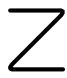
\includegraphics[keepaspectratio]{images/part001_11d71cd9.jpg}}

Remarks. 1) There can be infinitely many integrals of a differential equation (1) taking the same value at a given point. For example, the scalar differential equation \(x' = 2\sqrt{|x|}\) has all the functions defined by

\[
\begin{array}{l l} u (t) = 0 & \text { for } \quad - \beta \leqslant t \leqslant \alpha \\ u (t) = - (t + \beta) ^ {2} & \text { for } \quad t \leqslant - \beta \\ u (t) = (t - \alpha) ^ {2} & \text { for } \quad t \geqslant \alpha \end{array}
\]

as integrals taking the value 0 at the point t = 0, for any positive numbers \(\alpha\) and \(\beta\) .

\begin{enumerate}
\def\labelenumi{\arabic{enumi})}
\setcounter{enumi}{1}
\tightlist
\item
  Peano's theorem no longer holds when \(\mathbf{E}\) is an arbitrary complete normed space of infinite dimension (IV, p.~204, exerc. 18).
\end{enumerate}

\subsection{COMPARISON OF APPROXIMATE SOLUTIONS}

In what follows, I and H denote, as above, an interval contained in R and an open set in the normed space E, respectively; \(t_{0}\) is a point of I.

DEFINITION 1. Given a positive real function \(t \mapsto k(t)\) defined on I, one says that a map \(\mathbf{f}\) from \(\mathrm{I} \times \mathrm{H}\) into E is Lipschitz with respect to the function \(k(t)\) if, for every \(\mathbf{x} \in \mathrm{H}\) , the function \(t \mapsto \mathbf{f}(t, \mathbf{x})\) is regulated on I, and if, for every \(t \in \mathrm{I}\) and every pair of points \(\mathbf{x}_1, \mathbf{x}_2\) of H, one has (the ``Lipschitz condition'')

\[
\left\| \mathbf {f} (t, \mathbf {x} _ {1}) - \mathbf {f} (t, \mathbf {x} _ {2}) \right\| \leqslant k (t) \left\| \mathbf {x} _ {1} - \mathbf {x} _ {2} \right\|.\tag{8}
\]

We shall say that \(\mathbf{f}\) is Lipschitz (without being more specific) on \(\mathrm{I} \times \mathrm{H}\) if it is Lipschitz on this set for some constant \(k \geqslant 0\) . It is immediate that a Lipschitz function on \(\mathrm{I} \times \mathrm{H}\) satisfies the hypotheses of lemma 1 of IV, p.~165 (the converse being false); when \(\mathbf{f}\) is Lipschitz (on \(\mathrm{I} \times \mathrm{H}\) ) one says that the differential equation

\[
\mathbf {x} ^ {\prime} = \mathbf {f} (t, \mathbf {x})\tag{1}
\]

is Lipschitz (on I × H).

Example. When E = R and H is an interval in R, if the function \(f(t, x)\) admits a partial derivative \(f_{x}^{\prime}\) (II, p.~74) at every point \((t, x)\) of I × H, such that \(|f_{x}^{\prime}(t, x)| \leqslant k(t)\) on I × H, then condition (8) is satisfied, by the mean value theorem; we shall see later how this example generalizes to the case where E is an arbitrary normed space.

If f is Lipschitz on \(I \times H\) then f is bounded on \(J \times S\) for every compact subinterval \(J \subset I\) and every open ball \(S \subset H\) . Thus prop. 3 (IV, p.~166) can be applied, and demonstrates the existence of approximate solutions of equation (1). But we also have the following proposition, which allows us to compare two approximate solutions:

PROPOSITION 5. Let \(k(t)\) be a real regulated function and \(>0\) on I, and let \(\mathbf{f}(t, \mathbf{x})\) be a function that is defined and Lipschitz with respect to \(k(t)\) on \(\mathrm{I} \times \mathrm{H}\) . If \(\mathbf{u}\) and \(\mathbf{v}\) are two approximate solutions of (1), to within \(\varepsilon_1\) and \(\varepsilon_2\) respectively, defined on I with values in H, then, for all \(t \in \mathrm{I}\) such that \(t \geqslant t_0\) ,

\[
\left\| \mathbf {u} (t) - \mathbf {v} (t) \right\| \leqslant \left\| \mathbf {u} \left(t _ {0}\right) - \mathbf {v} \left(t _ {0}\right) \right\| \Phi (t) + \left(\varepsilon_ {1} + \varepsilon_ {2}\right) \Psi (t)\tag{9}
\]

where

\[
\left\{ \begin{array}{l} \Phi (t) = 1 + \int_ {t _ {0}} ^ {t} k (s) \exp \left(\int_ {s} ^ {t} k (\tau) d \tau\right) d s \\ \Psi (t) = t - t _ {0} + \int_ {t _ {0}} ^ {t} (s - t _ {0}) k (s) \exp \left(\int_ {s} ^ {t} k (\tau) d \tau\right) d s. \end{array} \right.\tag{10}
\]

From the relation \(\left\| \mathbf{u}'(t) - \mathbf{f}(t, \mathbf{u}(t)) \right\| \leqslant \varepsilon_1\) , valid on the complement of a countable set, one deduces, from the mean value theorem, that

\[
\left\| \mathbf {u} (t) - \mathbf {u} (t _ {0}) - \int_ {t _ {0}} ^ {t} \mathbf {f} (s, \mathbf {u} (s)) d s \right\| \leqslant \varepsilon_ {1} (t - t _ {0})
\]

and similarly

\[
\left\| \mathbf {v} (t) - \mathbf {v} (t _ {0}) - \int_ {t _ {0}} ^ {t} \mathbf {f} (s, \mathbf {v} (s)) d s \right\| \leqslant \varepsilon_ {2} (t - t _ {0})
\]

whence

\[
\begin{array}{l} \| \mathbf {u} (t) - \mathbf {v} (t) \| \leqslant \| \mathbf {u} (t _ {0}) - \mathbf {v} (t _ {0}) \| \\ \qquad + \left\| \int_ {t _ {0}} ^ {t} (\mathbf {f} (s, \mathbf {u} (s)) - \mathbf {f} (s, \mathbf {v} (s))) d s \right\| + (\varepsilon_ {1} + \varepsilon_ {2}) (t - t _ {0}). \end{array}
\]

By the Lipschitz condition (8) one has

\[
\begin{array}{r l} \left\| \int_ {t _ {0}} ^ {t} (\mathbf {f} (s, \mathbf {u} (s)) - \mathbf {f} (s, \mathbf {v} (s))) d s \right\| & \leqslant \int_ {t _ {0}} ^ {t} \| \mathbf {f} (s, \mathbf {u} (s)) - \mathbf {f} (s, \mathbf {v} (s)) \| d s \\ & \leqslant \int_ {t _ {0}} ^ {t} k (s) \| \mathbf {u} (s) - \mathbf {v} (s) \| d s \end{array}
\]

whence, putting \(w(t) = \|\mathbf{u}(t) - \mathbf{v}(t)\|\) ,

\[
w (t) \leqslant w \left(t _ {0}\right) + \left(\varepsilon_ {1} + \varepsilon_ {2}\right) \left(t - t _ {0}\right) + \int_ {t _ {0}} ^ {t} k (s) w (s) d s.\tag{11}
\]

The proposition is thus a consequence of the following lemma:

Lemma 2. If \(w\) is a continuous real function on the interval \([t_0, t_1]\) and satisfies the inequality

\[
w (t) \leqslant \varphi (t) + \int_ {t _ {0}} ^ {t} k (s) w (s) d s\tag{12}
\]

where \(\varphi\) is a regulated function \(\geqslant 0\) on \([t_0, t_1]\) , then, for \(t_0 \leqslant t \leqslant t_1\) ,

\[
w (t) \leqslant \varphi (t) + \int_ {t _ {0}} ^ {t} \varphi (s) k (s) \exp \left(\int_ {s} ^ {t} k (\tau) d \tau\right) d s.\tag{13}
\]

Put \(y(t) = \int_{t_0}^{t} k(s)w(s)ds\) ; the relation (12) implies that

\[
y ^ {\prime} (t) - k (t) y (t) \leqslant \varphi (t) k (t)\tag{14}
\]

on the complement of a countable set.

Put \(z(t) = y(t)\exp \left(-\int_{t_0}^t k(s)ds\right)\) ; then (14) is equivalent to

\[
z ^ {\prime} (t) \leqslant \varphi (t) k (t) \exp \left(- \int_ {t _ {0}} ^ {t} k (s) d s\right).
\]

On applying the mean value theorem (I, p.~15, th. 2) to this inequality, and noting that \(z(t_0) = 0\) , we obtain

\[
z (t) \leqslant \int_ {t _ {0}} ^ {t} \varphi (s) k (s) \exp \left(- \int_ {t _ {0}} ^ {s} k (\tau) d \tau\right) d s
\]

whence

\[
y (t) \leqslant \int_ {t _ {0}} ^ {t} \varphi (s) k (s) \exp \left(\int_ {s} ^ {t} k (\tau) d \tau\right) d s
\]

and since \(w(t) \leqslant \varphi(t) + y(t)\) one thus obtains (13).

COROLLARY. Let f be a Lipschitz function for the constant k \textgreater{} 0, defined on I × H. If u and v are two approximate solutions of (1) to within \(\varepsilon_{1}\) and \(\varepsilon_{2}\) respectively, defined on I and taking their values in H, then, for all \(t \in I\) ,

\[
\| \mathbf {u} (t) - \mathbf {v} (t) \| \leqslant \| \mathbf {u} (t _ {0}) - \mathbf {v} (t _ {0}) \| e ^ {k | t - t _ {0} |} + (\varepsilon_ {1} + \varepsilon_ {2}) \frac {e ^ {k | t - t _ {0} |} - 1}{k}.\tag{15}
\]

This inequality is in fact an immediate consequence of (9) when \(t \geqslant t_0\) ; to prove it for \(t \leqslant t_0\) it suffices to apply it to the equation

\[
{\frac {d \mathbf {x}}{d s}} = - \mathbf {f} (- s, \mathbf {x})
\]

obtained from (1) by the change of variable t = -s.

Remarks. 1) When k = 0 the inequality (15) is replaced by the inequality

\[
\left\| \mathbf {u} (t) - \mathbf {v} (t) \right\| \leqslant \left\| \mathbf {u} \left(t _ {0}\right) - \mathbf {v} \left(t _ {0}\right) \right\| + \left(\varepsilon_ {1} + \varepsilon_ {2}\right) | t - t _ {0} |
\]

whose proof is immediate.

\begin{enumerate}
\def\labelenumi{\arabic{enumi})}
\setcounter{enumi}{1}
\tightlist
\item
  When E is of finite dimension, and f is Lipschitz on \(I \times H\) , one can show the existence of approximate solutions of (1) (IV, p.~166, prop. 3) without using the axiom of choice (IV, p.~199, exerc. 1 b)).
\end{enumerate}

PROPOSITION 6. Let f and g be two functions defined on I × H, satisfying the hypotheses of lemma 1 of IV, p.~165, and such that, on I × H,

\[
\left\| \mathbf {f} (t, \mathbf {x}) - \mathbf {g} (t, \mathbf {x}) \right\| \leqslant \alpha .\tag{16}
\]

Suppose further that \(\mathbf{g}\) is Lipschitz for the constant \(k > 0\) on \(\mathrm{I} \times \mathrm{H}\) . In these circumstances, if \(\mathbf{u}\) is an approximate solution of \(\mathbf{x}' = \mathbf{f}(t, \mathbf{x})\) to within \(\varepsilon_1\) , defined on \(\mathrm{I}\) , with values in \(\mathrm{H}\) , and \(\mathbf{v}\) is an approximate solution of \(\mathbf{x}' = \mathbf{g}(t, \mathbf{x})\) to within \(\varepsilon_2\) , defined on \(\mathrm{I}\) , with values in \(\mathrm{H}\) , then, for all \(t \in \mathrm{I}\)

\[
\| \mathbf {u} (t) - \mathbf {v} (t) \| \leqslant \| \mathbf {u} (t _ {0}) - \mathbf {v} (t _ {0}) \| e ^ {k | t - t _ {0} |} + (\alpha + \varepsilon_ {1} + \varepsilon_ {2}) \frac {e ^ {k | t - t _ {0} |} - 1}{k}.\tag{17}
\]

Indeed

\[
\left| \left| \mathbf {u} ^ {\prime} (t) - \mathbf {g} (t, \mathbf {u} (t)) \right| \right| \leqslant \alpha + \varepsilon_ {1}
\]

for all t in the complement in I of a countable subset of I; in other words, u is an approximate solution of \(\mathbf{x}^{\prime} = \mathbf{g}(t, \mathbf{x})\) to within \(\alpha + \varepsilon_{1}\) , so the inequality (17) follows on applying prop. 5 of IV, p.~169.

\subsection{EXISTENCE AND UNIQUENESS OF SOLUTIONS OF LIPSCHITZ AND LOCALLY LIPSCHITZ EQUATIONS}

THEOREM 1 (Cauchy). Let \(\mathbf{f}\) be a Lipschitz function on \(\mathrm{I} \times \mathrm{H}\) , let \(\mathrm{J}\) be a compact subinterval of \(\mathrm{I}\) , not reducing to a single point, \(t_0\) a point of \(\mathrm{J}\) , \(\mathrm{S}\) an open ball with centre \(\mathbf{x}_0\) and radius \(r\) , contained in \(\mathrm{H}\) , and \(\mathrm{M}\) the least upper bound of \(\| \mathbf{f}(t, \mathbf{x})\|\) on \(\mathrm{J} \times \mathrm{S}\) . In these circumstances, for every compact interval \(\mathrm{K}\) that does not reduce to a single point and is contained in the intersection of \(\mathrm{J}\) with \(]t_0 - r / M\) , \(t_0 + r / M[\) , and contains \(t_0\) , there exists one and only one solution of the differential equation \(\mathbf{x}' = \mathbf{f}(t, \mathbf{x})\) defined on \(\mathrm{K}\) , with values in \(\mathrm{S}\) , and equal to \(\mathbf{x}_0\) at the point \(t_0\) .

Indeed, for \(\varepsilon > 0\) sufficiently small, the set \(F_{\varepsilon}\) of approximate solutions of (1) to within \(\varepsilon\) , defined on K, with values in S, and equal to \(x_{0}\) at the point \(t_{0}\) , is not empty (IV, p.~166, prop. 3); further, if u and v belong to \(F_{\varepsilon}\) then, by (15) (IV, p.~170)

\[
\| \mathbf {u} (t) - \mathbf {v} (t) \| \leqslant 2 \varepsilon \frac {e ^ {k | t - t _ {0} |} - 1}{k}
\]

for all \(t \in K\) , so the sets \(F_{\varepsilon}\) form a filter base G which converges uniformly on K to a continuous function w, equal to \(x_{0}\) at \(t_{0}\) ; also w takes values in S, since, for \(\varepsilon\) small enough, the functions \(u \in F_{\varepsilon}\) take their values in a closed ball contained in S. Since \(\mathbf{f}(t, \mathbf{u}(t))\) tends uniformly on K to \(\mathbf{f}(t, \mathbf{w}(t))\) along G, w satisfies equation (6) of IV, p.~165, so is a solution of (1). The uniqueness of the solution follows immediately from inequality (15) of IV, p.~170 where one takes \(\varepsilon_{1} = \varepsilon_{2} = 0\) and \(\mathbf{u}(t_{0}) = \mathbf{v}(t_{0})\) .

We shall say that a function \(\mathbf{f}\) defined on \(\mathrm{I} \times \mathrm{H}\) is locally Lipschitz if, for every point \((t, \mathbf{x})\) of \(\mathrm{I} \times \mathrm{H}\) , there exists a neighbourhood \(\mathrm{V}\) of \(t\) (with respect to \(\mathrm{I}\) ) and a neighbourhood \(\mathrm{S}\) of \(\mathbf{x}\) such that \(\mathbf{f}\) is Lipschitz on \(\mathrm{V} \times \mathrm{S}\) (for a constant \(k\) depending on \(\mathrm{V}\) and \(\mathrm{S}\) ). By the Borel-Lebesgue theorem, for every compact interval \(\mathrm{J} \subset \mathrm{I}\) and every point \(\mathbf{x}_0 \in \mathrm{H}\) there exists an open ball \(\mathrm{S}\) with centre \(\mathbf{x}_0\) , contained in \(\mathrm{H}\) , such that \(\mathbf{f}\) is Lipschitz on \(\mathrm{J} \times \mathrm{S}\) ; thus \(\mathbf{f}\) satisfies the hypotheses of lemma 1 of IV, p.~3. When \(\mathbf{f}\) is locally Lipschitz on \(\mathrm{I} \times \mathrm{H}\) we shall say that the equation \(\mathbf{x}' = \mathbf{f}(t, \mathbf{x})\) is locally Lipschitz on \(\mathrm{I} \times \mathrm{H}\) .

We shall generalize and clarify th. 1 of IV, p.~10 for locally Lipschitz equations; we restrict ourselves to the case where \(t_0\) is the left endpoint of the interval I; one can pass easily to the case where \(t_0\) is an arbitrary point of I (cf.~IV, §IV ??, p.~9, corollary).

THEOREM 2. Let \(\mathbf{I} \subset \mathbf{R}\) be an interval (not reducing to a single point) with left-hand endpoint \(t_0 \in \mathbf{I}\) , let \(\mathbf{H}\) be a nonempty open set in \(\mathbf{E}\) , and \(\mathbf{f}\) a locally Lipschitz function on \(\mathbf{I} \times \mathbf{H}\) .

\(1^{\circ}\) For \(\mathbf{x}_0\in \mathrm{H}\) there exists a largest interval \(\mathbf{J}\subset \mathbf{I}\) , with left-hand endpoint \(t_0\in \mathbf{J}\) , on which there exists an integral \(\mathbf{u}\) of the equation \(\mathbf{x}' = \mathbf{f}(t,\mathbf{x})\) taking values in H and equal to \(\mathbf{x}_0\) at the point \(t_0\) ; this integral is unique.

\(2^{\circ}\) If \(\mathrm{J} \neq \mathrm{I}\) then \(\mathrm{J}\) is a half-open interval \([t_0, \beta[\) of finite length; further, for every compact subset \(\mathbf{K} \subset \mathbf{H}\) the set \(\overline{\mathbf{u}}^{-1}(\mathbf{K})\) is a compact subset of \(\mathbf{R}\) .

\(3^{\circ}\) If \(\mathbf{J}\) is bounded, and if \(\mathbf{f}(t,\mathbf{u}(t))\) is bounded on \(\mathbf{J}\) , then \(\mathbf{u}(t)\) has a left limit \(\mathbf{c}\) at the right-hand endpoint of \(\mathbf{J}\) ; further, if \(\mathbf{J} \neq \mathbf{I}\) then \(\mathbf{c}\) is a boundary point of \(\mathbf{H}\) in \(\mathbf{E}\) .

\(1^{\circ}\) Let \(\mathfrak{M}\) be the set of intervals L (not reducing to a single point) with left-hand endpoint \(t_0 \in L\) which are contained in I and are such that on L there is a solution of (1) (IV, p.~163) with values in H and equal to \(\mathbf{x}_0\) at \(t_0\) ; by th. 1 (IV, p.~171) the set \(\mathfrak{M}\) is not empty. Let L and L' be two intervals belonging to \(\mathfrak{M}\) , and suppose, for example, that L \(\subset\) L'; if u and v are two integrals of (1) defined respectively on L and L', with values in H, and equal to \(\mathbf{x}_0\) at \(t_0\) , we shall see that v is an extension of u. Indeed, let \(t_1\) be the supremum of the set of \(t \in L\) such that \(\mathbf{u}(s) = \mathbf{v}(s)\) for \(t_0 \leqslant s \leqslant t\) ; we shall show that \(t_1\) is the right-hand endpoint of L. If this were not so, we would have \(\mathbf{u}(t_1) = \mathbf{v}(t_1)\) by continuity, and \(\mathbf{x}_1 = \mathbf{u}(t_1)\) would belong to H; since f is locally Lipschitz, th. 1 shows that there can exist only one integral of (1) defined on a neighbourhood of \(t_1\) with values in H and equal to \(\mathbf{x}_1\) at \(t_1\) ; it is therefore a contradiction to suppose that \(t_1\) is not the right-hand endpoint of L. We now see that if J is the union of the intervals L \(\in\) M there exists one and only one integral u of (1), defined on J, with values in H and equal to \(\mathbf{x}_0\) at \(t_0\) .

\(2^{\circ}\) Suppose that \(\mathrm{J} \neq \mathrm{I}\) and let \(\beta\) be the right endpoint of \(\mathrm{J}\) ; if \(\beta\) is the right-hand endpoint of \(\mathrm{I}\) then \(\beta \in \mathrm{I}\) (so \(\beta\) is finite) and \(\mathrm{J} = [t_0, \beta[\) by hypothesis. Suppose then that \(\beta\) is not the right-hand endpoint of \(\mathrm{I}\) ; if \(\beta \in \mathrm{J}\) then \(\mathbf{u}(\beta) = \mathbf{c}\) belongs to \(\mathrm{H}\) ; by th. 1 there exists an integral of (1) with values in \(\mathrm{H}\) , defined on an interval

\[
[ \beta , \beta_ {1} [ \subset I
\]

and equal to \(\mathbf{c}\) at \(\beta\) ; then \(\mathrm{J}\) would not be the largest of the intervals in \(\mathfrak{M}\) , which is absurd; so \(\mathrm{J} = [t_0, \beta[\) .

If K is a compact subset of H then \(\overline{\mathbf{u}}^{-1}(\mathbf{K})\) is closed in J; we shall see that there exists a \(\gamma\in J\) such that \(\overline{\mathbf{u}}^{-1}(\mathbf{K})\) is contained in \([t_{0},\gamma]\) , which will prove that \(\overline{\mathbf{u}}^{-1}(\mathbf{K})\) is compact. If not, there would be a point \(c\in K\) such that \((\beta,\mathbf{c})\) is a cluster point of the set of points \((t,\mathbf{u}(t))\) such that \(t<\beta\) and \(\mathbf{u}(t)\in\mathbf{K}\) . Since \(\beta\in I\) and \(c\in H\) there exists a neighbourhood V of \(\beta\) in I, and an open ball S with centre c and radius r contained in H, such that f is Lipschitz and bounded on V×S; let M be the supremum of \(\|\mathbf{f}(t,\mathbf{x})\|\) over this set. By hypothesis there exists a \(t_{1}\in J\) such that \(\beta-t_{1}<r/2M\) , \(t_{1}\in V\) and \(\|\mathbf{u}(t_{1})-\mathbf{c}\|\leqslant r/2\) ; th. 1 shows that there exists one and only one integral of (1), with values in H, defined on an interval \([t_{1},t_{2}]\) containing \(\beta\) , and equal to \(\mathbf{u}(t_{1})\) at \(t_{1}\) ; since this interval coincides with u on the interval \([t_{1},\beta[\) it follows that \(J=[t_{0},\beta[\) is not the largest interval in M, which is absurd.

\(3^{\circ}\) Suppose that \(\mathbf{J}\) is bounded and that \(\| \mathbf{f}(t,\mathbf{u}(t))\| \leqslant M\) on \(\mathbf{J}\) ; then \(\| \mathbf{u}'(t)\| \leqslant \mathbf{M}\) on the complement of a countable subset of \(\mathbf{J}\) ; then, by the mean value theorem, \(\| \mathbf{u}(s) - \mathbf{u}(t)\| \leqslant \mathbf{M} |s - t|\) for any \(s\) and \(t\) in \(\mathbf{J}\) ; by the Cauchy criterion, \(\mathbf{u}\) has a left limit \(\mathbf{c}\) at the right endpoint \(\beta\) of \(\mathbf{J}\) . If \(\mathbf{J} \neq \mathbf{I}\) then \(\mathbf{c}\) cannot belong to \(\mathbf{H}\) , for on extending \(\mathbf{u}\) by continuity at \(\beta\) , \(\mathbf{u}\) would be an integral of (1) with values in \(\mathbf{H}\) , defined on an interval \([t_0, \beta]\) and equal to \(\mathbf{x}_0\) at \(t_0\) ; then one would have \(\mathbf{J} = [t_0, \beta]\) , contradicting what we have seen in \(2^{\circ}\) .

COROLLARY 1. If H = E and J ≠ I then \(\mathbf{f}(t, \mathbf{u}(t))\) is not bounded on J; if, further, E is finite dimensional, then \(\| \mathbf{u}(t) \|\) has left limit \(+\infty\) at the right-hand endpoint of J.

The first part is an immediate consequence of the third part of th. 2. If E is finite dimensional then every closed ball \(S \subset E\) is compact, so the second part of th. 2 shows that there exists a \(\gamma \in J\) such that \(\mathbf{u}(t) \notin \mathbf{S}\) for \(t > \gamma\) .

If E is finite dimensional it can happen that \(J \neq I\) but that \(\|\mathbf{u}(t)\|\) remains bounded as t tends to the right-hand endpoint of J (IV, p.~200, exerc. 5).

COROLLARY 2. If, on I × H, the function f is Lipschitz with respect to a regulated function k(t), and if the right-hand endpoint β of J belongs to I, then u has a left limit at β; if H = E and if f is Lipschitz with respect to a regulated function k(t) on I × E, then J = I.

Indeed, if \(\beta \in \mathbf{I}\) , there exists a compact neighbourhood \(\mathrm{V}\) of \(\beta\) in \(\mathbf{I}\) , such that \(\mathbf{f}(t, \mathbf{x}_0)\) and \(k(t)\) are bounded on \(\mathrm{V}\) ; then \(\| \mathbf{f}(t, \mathbf{x}) \| \leqslant m \| x \| + h\) ( \(m\) and \(h\) constant)

on \(V \times H\) , whence \(\left\|\mathbf{u}^{\prime}(t)\right\| \leqslant m \left\|\mathbf{u}(t)\right\| + h\) on the complement of a countable subset of \(V \cap J\) , so that \(\left\|\mathbf{u}(t)\right\| \leqslant m \int_{t_{0}}^{t} \left\|\mathbf{u}(s)\right\| ds + q\) (q constant) on \(V \cap J\) ; lemma 2 (IV, p.~170) shows that \(\left\|\mathbf{u}(t)\right\| \leqslant c e^{mt} + d\) (c and d constant) on \(V \cap J\) , and thus \(\mathbf{f}(t, \mathbf{u}(t))\) remains bounded on J, and the corollary results from th. 2 of IV, p.~172.

Examples. 1) For a differential equation of the form \(\mathbf{x}' = \mathbf{g}(t)\) , where \(\mathbf{g}\) is regulated on I, every integral \(\mathbf{u}\) is clearly defined on all of I. One should note that \(\mathbf{u}\) can be bounded on I without \(\mathbf{g}(t)\) being so.

\begin{enumerate}
\def\labelenumi{\arabic{enumi})}
\setcounter{enumi}{1}
\item
  For the scalar equation \(x' = \sqrt{1 - x^2}\) one has \(I = R\) , \(H = ] - 1, +1[\) . If one takes \(t_0 = x_0 = 0\) the corresponding integral is \(\sin t\) on the largest interval containing 0 where the derivative of \(\sin t\) is positive, that is to say, on \(] - \pi / 2, +\pi / 2[\) ; at the endpoints of this interval the integral tends to an endpoint of \(H\) .
\item
  For the scalar equation \(x' = 1 + x^{2}\) one has I = H = R; the integral that vanishes at t = 0 is \(\tan t\) , and the largest interval containing 0 where this function is continuous is \(J = ] - \pi/2, +\pi/2[\) ; and \(|\tan t|\) tends to \(+\infty\) at the endpoints of J (cf.~IV, p.~173, cor. 1).
\item
  For the scalar equation \(x' = \sin tx\) one has I = H = R and the right-hand side is bounded on I × H, so (IV, p.~173, cor. 1) every integral is defined on all of R.
\end{enumerate}

\subsection{CONTINUITY OF INTEGRALS AS FUNCTIONS OF A PARAMETER}

Prop. 6 (IV, p.~171) shows that when a differential equation

\[
\mathbf {x} ^ {\prime} = \mathbf {f} (t, \mathbf {x})
\]

is ``close'' to a Lipschitz equation \(\mathbf{x}^{\prime} = \mathbf{g}(t, \mathbf{x})\) and when one supposes that both equations have an approximate solution on the same interval, then these approximate solutions are ``close''; we shall clarify this result by showing that the existence of solutions of the Lipschitz equation \(\mathbf{x}^{\prime} = \mathbf{g}(t, \mathbf{x})\) on an interval implies that of approximate solutions of \(\mathbf{x}^{\prime} = \mathbf{f}(t, \mathbf{x})\) on the same interval, so long as, on the latter, the values of the solution of \(\mathbf{x}^{\prime} = \mathbf{g}(t, \mathbf{x})\) are not ``too close'' to the boundary of H.

PROPOSITION 7. Let f and g be two functions defined on I × H, satisfying the hypotheses of lemma 1 of IV. p.~165, and such that, on I × H

\[
\left\| \mathbf {f} (t, \mathbf {x}) - \mathbf {g} (t, \mathbf {x}) \right\| \leqslant \alpha .\tag{16}
\]

Suppose further that \(\mathbf{g}\) is Lipschitz with respect to a constant \(k > 0\) on \(\mathrm{I} \times \mathrm{H}\) and that \(\mathbf{f}\) is locally Lipschitz on \(\mathrm{I} \times \mathrm{H}\) , or that \(\mathrm{E}\) is finite dimensional. Let \((t_0, \mathbf{x}_0)\) be a point of \(\mathrm{I} \times \mathrm{H}\) , \(\mu\) a number \(>0\) , and

\[
\varphi (t) = \mu e ^ {k (t - t _ {0})} + \alpha \frac {e ^ {k (t - t _ {0})} - 1}{k}.
\]

Let \(\mathbf{u}\) be an integral of the equation \(\mathbf{x}' = \mathbf{g}(t, \mathbf{x})\) defined on an interval \(\mathrm{K} = [t_0, b[\) contained in I, equal to \(\mathbf{x}_0\) at the point \(t_0\) , and such that for all \(t \in \mathrm{K}\) the closed ball with centre \(\mathbf{u}(t)\) and radius \(\varphi(t)\) is contained in H. Under these conditions, for every \(\mathbf{y} \in \mathrm{H}\) such that \(\| \mathbf{y} - \mathbf{x}_0 \| \leqslant \mu\) there exists an integral \(\mathbf{v}\) of \(\mathbf{x}' = \mathbf{f}(t, \mathbf{x})\) , defined on K, with values in H, and equal to \(\mathbf{y}\) at the point \(t_0\) ; moreover, \(\| \mathbf{u}(t) - \mathbf{v}(t) \| \leqslant \varphi(t)\) on K.

Let M be the family of integrals of \(\mathbf{x}^{\prime} = \mathbf{f}(t, \mathbf{x})\) each of which takes its values in H, is equal to y at \(t_{0}\) , and is defined on a half-open interval \([t_{0}, \tau[\) contained in I (depending on the interval considered). By th. 1 of IV, p.~171 (when f is locally Lipschitz) or IV, p.~167 corollary (when E is finite dimensional), M is not empty, and the same reasoning as in prop. 3 of IV, p.~166 shows that M is inductive for the order ``v is a restriction of w''. Let \(v_{0}\) be a maximal element of M and \([t_{0}, t_{1}[\) the interval of definition of \(v_{0}\) ; by prop. 6 of IV, p.~171, it all comes down to proving that \(t_{1} \geqslant b\) . If not, one would have

\[
\left\| \mathbf {u} (t) - \mathbf {v} _ {0} (t) \right\| \leqslant \varphi (t)
\]

on the interval \([t_0, t_1[\) by prop. 6; now on the compact interval \([t_0, t_1]\) the regulated function \(\mathbf{g}(t, \mathbf{u}(t))\) is bounded, so the function \(\mathbf{g}(t, \mathbf{v}_0(t))\) is bounded on the interval \([t_0, t_1[\) , for \(\| \mathbf{g}(t, \mathbf{v}_0(t)) \| \leqslant \| \mathbf{g}(t, \mathbf{u}(t)) \| + k\varphi(t)\) on this interval. Since \(\mathbf{v}_0\) is an approximate solution of \(\mathbf{x}' = \mathbf{g}(t, \mathbf{x})\) to within \(\alpha\) on \([t_0, t_1[\) there exists a number \(M > 0\) such that \(\| \mathbf{v}_0'(t) \| \leqslant M\) on this interval, except at the points of a countable set; the mean value theorem now shows that \(\| \mathbf{v}_0(s) - \mathbf{v}_0(t) \| \leqslant M |s - t|\) for every pair of points \(s\) , \(t\) of \([t_0, t_1[\) , so (by Cauchy's criterion) \(\mathbf{v}_0(t)\) has a left limit \(\mathbf{c}\) at the point \(t_1\) , and, by continuity, one has \(\| \mathbf{c} - \mathbf{u}(t_1) \| \leqslant \varphi(t_1)\) , and so \(\mathbf{c} \in H\) . Now one sees, from IV, p.~171, th. 1 or IV, p.~167, corollary, that there exists an integral of \(\mathbf{x}' = \mathbf{f}(t, \mathbf{x})\) defined on an interval \([t_1, t_2[\) and equal to \(\mathbf{c}\) at \(t_1\) , which contradicts the definition of \(\mathbf{v}_0\) .

THEOREM 3. Let F be a topological space and let f be a map from I × H × F into E such that, for every \(\xi \in F\) , the function \((t, \mathbf{x}) \mapsto \mathbf{f}(t, \mathbf{x}, \xi)\) is Lipschitz on I × H, and such that, when \(\xi\) tends to \(\xi_{0}\) , \(\mathbf{f}(t, \mathbf{x}, \xi)\) tends uniformly to \(\mathbf{f}(t, \mathbf{x}, \xi_{0})\) on I × H. Let \(\mathbf{u}_{0}(t)\) be an integral of \(\mathbf{x}' = \mathbf{f}(t, \mathbf{x}, \xi_{0})\) defined on an interval J = {[}t₀, b{[} contained in I, with values in H, and equal to \(x_{0}\) at t₀. For every compact interval {[}t₀, t₁{]} contained in J there exists a neighbourhood V of \(\xi_{0}\) in F such that, for every \(\xi \in V\) , the equation \(\mathbf{x}' = \mathbf{f}(t, \mathbf{x}, \xi)\) has an integral (and only one) \(\mathbf{u}(t, \xi)\) defined on {[}t₀, t₁{]}, with values in H and equal to \(x_{0}\) at t₀; moreover, when \(\xi\) tends to \(\xi_{0}\) the solution \(\mathbf{u}(t, \xi)\) tends uniformly to \(\mathbf{u}_{0}(t)\) on {[}t₀, t₁{]}.

Indeed, let r \textgreater{} 0 be such that for \(t_{0} \leqslant t \leqslant t_{1}\) the closed ball with centre \(\mathbf{u}_{0}(t)\) and radius r is contained in H; if \(\mathbf{f}(t, \mathbf{x}, \xi)\) is Lipschitz with respect to the constant k \textgreater{} 0 on I × H we take \(\alpha\) small enough that \(\alpha \frac{e^{k(t_{1}-t_{0})} - 1}{k} < r\) ; taking V such that, for every \(\xi \in V\) , one has \(\|f(t, \mathbf{x}, \xi) - f(t, \mathbf{x}, \xi_{0})\| \leqslant \alpha\) on I × H, one can apply prop. 7 of IV, p.~174; moreover,

\[
\| \mathbf {u} (t, \xi) - \mathbf {u} _ {0} (t) \| \leqslant \alpha \frac {e ^ {k \left(t _ {1} - t _ {0}\right)} - 1}{k}
\]

on \([t_{0}, t_{1}]\) , which completes the proof of the theorem.

Remark. When H = E and the condition (16) of IV, p.~174 is satisfied on I × E, prop. 7 of IV, p.~174 applies to every solution u of \(\mathbf{x}' = \mathbf{g}(t, \mathbf{x})\) on any interval where this solution is defined; one may even assume that \(\mathbf{g}(t,\mathbf{x})\) is Lipschitz with respect to a regulated function \(k(t)\) though not necessarily bounded on this interval.

\subsection{DEPENDENCE ON INITIAL CONDITIONS}

Let \(\mathbf{x}^{\prime}=\mathbf{f}(t,\mathbf{x})\) be a locally Lipschitz equation on \(I\times H\) ; by th. 2 (IV, p.~172), for every point \((t_{0},\mathbf{x}_{0})\) of \(I\times H\) there exists a largest interval \(J(t_{0},\mathbf{x}_{0})\subset I\) , not reducing to a single point, containing \(t_{0}\) , and on which there exists an integral (and only one) of this equation, equal to \(x_{0}\) at \(t_{0}\) ; we shall clarify the manner in which this integral, and the interval \(J(t_{0},\mathbf{x}_{0})\) where it is defined, depend on the point \((t_{0},\mathbf{x}_{0})\) .

THEOREM 4. Let \(\mathbf{f}\) be a locally Lipschitz function on \(\mathrm{I} \times \mathrm{H}\) and \((a, \mathbf{b})\) an arbitrary point of \(\mathrm{I} \times \mathrm{H}\) .

\(1^{\circ}\) There exist an interval \(\mathbf{K} \subset \mathbf{I}\) , a neighbourhood of \(a\) in \(\mathbf{I}\) , and a neighbourhood \(\mathbf{V}\) of \(\mathbf{b}\) in \(\mathbf{H}\) such that, for every point \((t_0, \mathbf{x}_0)\) of \(\mathbf{K} \times \mathbf{V}\) , there exists an integral (and only one) \(\mathbf{u}(t, t_0, \mathbf{x}_0)\) defined on \(\mathbf{K}\) , with values in \(\mathbf{H}\) and equal to \(\mathbf{x}_0\) at the point \(t_0\) (in other words, \(J(t_0, \mathbf{x}_0) \supset \mathbf{K}\) for all \((t_0, \mathbf{x}_0) \in \mathbf{K} \times \mathbf{V}\) ).

\(2^{\circ}\) The map \((t,t_0,\mathbf{x}_0)\mapsto \mathbf{u}(t,t_0,\mathbf{x}_0)\) of \(\mathrm{K}\times \mathrm{K}\times \mathrm{V}\) into H is uniformly continuous.

\(3^{\circ}\) There exists a neighbourhood \(\mathbf{W} \subset \mathbf{V}\) of \(\mathbf{b}\) in \(\mathbf{H}\) such that, for every point

\[
(t, t _ {0}, \mathbf {x} _ {0}) \in \mathrm{K} \times \mathrm{K} \times \mathrm{W},
\]

the equation \(\mathbf{x}_{0} = \mathbf{u}(t_{0}, t, \mathbf{x})\) has a unique solution x on V equal to \(\mathbf{u}(t, t_{0}, \mathbf{x}_{0})\) (``resolution of the integral with respect to the constant of integration'').

\(1^{\circ}\) Let S be a ball with centre \(\mathbf{b}\) and radius \(r\) contained in H, and \(\mathrm{J}_0\) an interval contained in I, a neighbourhood of \(a\) in I, such that \(\mathbf{f}\) is bounded and Lipschitz (with respect to some constant \(k\) ) on \(\mathrm{J}_0 \times \mathrm{S}\) ; denote by M the supremum of \(\| \mathbf{f}(t, \mathbf{x})\|\) on \(\mathrm{J}_0 \times \mathrm{S}\) . Then there exist (IV, p.~171, th. 1) an interval \(\mathrm{J} \subset \mathrm{J}_0\) , a neighbourhood of \(a\) in I, and an integral \(\mathbf{v}\) of \(\mathbf{x}' = \mathbf{f}(t, \mathbf{x})\) defined on J, with values in S and equal to \(\mathbf{b}\) at \(a\) . We shall see that the open ball V with centre \(\mathbf{b}\) and radius \(r/2\) , and the intersection K of J with an interval \([a - l, a + l[\) , where \(l\) is small enough, are as required. Indeed, prop. 7 of IV, p.~174 (applied to the set \(\mathrm{J}_0 \times \mathrm{S}\) and the case where \(\alpha = 0\) ) shows that there exists an integral of \(\mathbf{x}' = \mathbf{f}(t, \mathbf{x})\) defined on K, with values in S, and equal to \(\mathbf{x}_0\) at a point \(t_0 \in \mathrm{K}\) , provided that

\[
\left\| \mathbf {v} (t) - \mathbf {b} \right\| + \left\| \mathbf {v} (t _ {0}) - \mathbf {x} _ {0} \right\| e ^ {k | t - t _ {0} |} <   r\tag{18}
\]

for every \(t \in \mathbf{K}\) . Now, by the mean value theorem, one has

\[
\| \mathbf {v} (t) - \mathbf {b} \| \leqslant \mathrm{M} | t - a | \leqslant \mathrm{M} l
\]

for every \(t \in \mathbf{K}\) ; since \(\| \mathbf{x}_0 - \mathbf{b} \| < r / 2\) one sees that it suffices to take \(l\) such that

\[
\mathbf {M} l + (\mathbf {M} l + r / 2) e ^ {2 k l} <   r\tag{19}
\]

for the relation (18) to be satisfied for every \((t, t_{0}, \mathbf{x}_{0})\) of \(K \times K \times V\) .

\(2^{\circ}\) By the mean value theorem we have

\[
\left\| \mathbf {u} (t _ {1}, t _ {0}, \mathbf {x} _ {0}) - \mathbf {u} (t _ {2}, t _ {0}, \mathbf {x} _ {0}) \right\| \leqslant \mathrm{M} \left| t _ {2} - t _ {1} \right|\tag{20}
\]

for all \(t_0, t_1, t_2\) in K and \(\mathbf{x}_0\) in V. Now prop. 5 (IV, p.~169) shows that

\[
\left\| \mathbf {u} (t, t _ {0}, \mathbf {x} _ {1}) - \mathbf {u} (t, t _ {0}, \mathbf {x} _ {2}) \right\| \leqslant e ^ {2 k t} \left\| \mathbf {x} _ {2} - \mathbf {x} _ {1} \right\|\tag{21}
\]

for every t and \(t_{0}\) in K, and \(x_{1}\) and \(x_{2}\) in V. Finally, if \(t_{1}\) and \(t_{2}\) are any two points in K,

\[
\left\| \mathbf {u} \left(t _ {1}, t _ {2}, \mathbf {x} _ {0}\right) - \mathbf {u} \left(t _ {2}, t _ {2}, \mathbf {x} _ {0}\right) \right\| \leqslant \mathrm{M} \left| t _ {2} - t _ {1} \right|
\]

by the mean value theorem, that is to say

\[
\left\| \mathbf {u} (t _ {1}, t _ {2}, \mathbf {x} _ {0}) - \mathbf {x} _ {0} \right\| \leqslant \mathbf {M} \left| t _ {2} - t _ {1} \right|;
\]

since \(\mathbf{u}(t, t_2, \mathbf{x}_0)\) is identical to the integral which takes the value \(\mathbf{u}(t_1, t_2, \mathbf{x}_0)\) at the point \(t_1\) , prop. 5 (IV, p.~169) shows that

\[
\left\| \mathbf {u} (t, t _ {1}, \mathbf {x} _ {0}) - \mathbf {u} (t, t _ {2}, \mathbf {x} _ {0}) \right\| \leqslant \mathrm{Me} ^ {2 k l} | t _ {2} - t _ {1} |\tag{22}
\]

for all \(t, t_{1}, t_{2}\) in \(\mathbf{K}\) and \(\mathbf{x}_{0}\) in \(\mathrm{V}\) . The three inequalities (20), (21) and (22) thus prove the uniform continuity of the map \((t, t_{0}, \mathbf{x}_{0}) \mapsto \mathbf{u}(t, t_{0}, \mathbf{x}_{0})\) on \(\mathrm{K} \times \mathrm{K} \times \mathrm{V}\) .

\(3^{\circ}\) By (20), we have \(\|\mathbf{u}(t, t_{0}, \mathbf{x}_{0}) - \mathbf{x}_{0}\| \leqslant \mathbf{M} |t - t_{0}| \leqslant 2\mathbf{M}l\) on

\[
\mathbf {K} \times \mathbf {K} \times \mathbf {V}.
\]

If \(l\) is taken small enough, so that \(2\mathrm{M}l < r / 4\) , one then sees that if \(\mathbf{x}_0\) is any point of the open ball \(\mathbf{W}\) with centre \(\mathbf{b}\) and radius \(r / 4\) , that \(\mathbf{u}(t,t_0,\mathbf{x}_0)\in \mathbf{V}\) for any \(t\) and \(t_0\) in \(\mathbf{K}\) . If \(\mathbf{x} = \mathbf{u}(t,t_0,\mathbf{x}_0)\) , the function \(s\mapsto \mathbf{u}(s,t,\mathbf{x})\) is then defined on \(\mathbf{K}\) and is equal to the integral of (1) which takes the value \(\mathbf{x}\) at the point \(t\) , that is, to \(\mathbf{u}(s,t_0,\mathbf{x}_0)\) ; in particular

\[
\mathbf {x} _ {0} = \mathbf {u} (t _ {0}, t _ {0}, \mathbf {x} _ {0}) = \mathbf {u} (t _ {0}, t, \mathbf {x}).
\]

Moreover, if \(y \in V\) is such that \(\mathbf{x}_{0} = \mathbf{u}(t_{0}, t, \mathbf{y})\) , then the integral \(s \mapsto \mathbf{u}(s, t, \mathbf{y})\) takes the value \(x_{0}\) at \(t_{0}\) so is identical to \(s \mapsto \mathbf{u}(s, t_{0}, \mathbf{x}_{0})\) , which consequently takes the value x at t, which shows that y = x and concludes the proof.

\section{LINEAR DIFFERENTIAL EQUATIONS}

\subsection{EXISTENCE OF INTEGRALS OF A LINEAR DIFFERENTIAL EQUATION}

Let E be a complete normed space over the field R, and J an interval in R, not reducing to a point. One says that the differential equation

\[
{\frac {d \mathbf {x}}{d t}} = \mathbf {f} (t, \mathbf {x})\tag{1}
\]

where \(\mathbf{f}\) is defined on \(\mathbf{J} \times \mathbf{E}\) , is a linear equation if, for every \(t \in \mathbf{J}\) , the map \(\mathbf{x} \mapsto \mathbf{f}(t, \mathbf{x})\) is a continuous affine linear map \(^1\) from E into itself; if one puts \(\mathbf{b}(t) = \mathbf{f}(t, 0)\) the map \(\mathbf{x} \mapsto \mathbf{f}(t, \mathbf{x}) - \mathbf{f}(t, 0) = \mathbf{f}(t, \mathbf{x}) - \mathbf{b}(t)\) is then a continuous linear map from E to itself; from now on we shall denote this map by \(A(t)\) and write \(A(t).\mathbf{x}\) , (or simply \(A(t)\mathbf{x}\) ) for its value at the point \(\mathbf{x} \in E\) ; thus the linear differential equation (1) may be written

\[
{\frac {d \mathbf {x}}{d t}} = A (t). \mathbf {x} + \mathbf {b} (t)\tag{2}
\]

where \(\mathbf{b}\) is a map from J into E; when \(\mathbf{b} = 0\) one says that the linear differential equation (2) is homogeneous.

Examples. 1) When E is of finite dimension n over R one can identify the endomorphism \(A(t)\) with its matrix \(\left(a_{ij}(t)\right)\) with respect to any basis of E (Alg., II, p.~343); when one identifies a vector \(x \in E\) with the column matrix \(\left(x_{j}\right)\) of its components with respect to the basis of E under consideration the expression \(A(t)\) .x conforms to the general conventions of Algebra (Alg., II, p.~343, prop. 2). In this case, equation (2) is equivalent to the system of scalar differential equations

\[
\frac {d x _ {i}}{d t} = \sum_ {j = 1} ^ {n} a _ {i j} (t) x _ {j} + b _ {i} (t) \quad (1 \leqslant i \leqslant n).\tag{3}
\]

\begin{enumerate}
\def\labelenumi{\arabic{enumi})}
\setcounter{enumi}{1}
\tightlist
\item
  Let \(\mathbf{G}\) be a complete normed algebra over \(\mathbf{R}\) , and \(\mathbf{a}(t)\) , \(\mathbf{b}(t)\) and \(\mathbf{c}(t)\) three maps from \(\mathbf{J}\) into \(\mathbf{G}\) ; the equation
\end{enumerate}

\[
\frac {d \mathbf {x}}{d t} = \mathbf {a} (t) \mathbf {x} + \mathbf {x b} (t) + \mathbf {c} (t)
\]

is a linear differential equation; here \(A(t)\) is the linear map \(\mathbf{x} \mapsto \mathbf{a}(t)\mathbf{x} + \mathbf{x}\mathbf{b}(t)\) of \(G\) to itself.

For every \(t \in J\) , \(A(t)\) is an element of the set \(\mathcal{L}(\mathrm{E})\) of continuous linear maps from E to itself (continuous endomorphisms of E); one knows (Gen.~Top., X, p.~298) that \(\mathcal{L}(\mathrm{E})\) , endowed with the norm \(\|U\| = \sup_{\|x\| \leqslant 1} \|Ux\|\) is a complete normed algebra over the field R, and that \(\|UV\| \leqslant \|U\|\) \(\|V\|\) .

Throughout this section we shall assume that the following conditions are satisfied:

\begin{enumerate}
\def\labelenumi{\alph{enumi})}
\item
  The map \(t \mapsto A(t)\) of \(\mathbf{J}\) into \(\mathcal{L}(\mathrm{E})\) is regulated.
\item
  The map \(t \mapsto \mathbf{b}(t)\) of J into E is regulated.
\end{enumerate}

When \(\mathrm{E}\) has dimension \(n\) , \(\mathcal{L}(\mathrm{E})\) is isomorphic to \(\mathbf{R}^{n^2}\) (as a topological vector space) and condition \(a\) ) means that each of the elements \(a_{ij}(t)\) of the matrix \(A(t)\) is a regulated function on \(\mathrm{J}\) .

Since \(\left\| A(t')\mathbf{x} - A(t)\mathbf{x}\right\| \leqslant \left\| A(t') - A(t)\right\| \| \mathbf{x}\|\) , the map

\[
t \mapsto A (t). \mathbf {x} + \mathbf {b} (t)
\]

is regulated for every \(\mathbf{x} \in \mathrm{E}\) ; further,

\[
\left\| A (t) \mathbf {x} _ {1} - A (t) \mathbf {x} _ {2} \right\| = \left\| A (t) \left(\mathbf {x} _ {1} - \mathbf {x} _ {2}\right) \right\| \leqslant \left\| A (t) \right\| \left\| \mathbf {x} _ {1} - \mathbf {x} _ {2} \right\|
\]

for any \(t \in J\) and \(x_{1}\) , \(x_{2}\) in E; in other words, the right-hand side of (2) satisfies the conditions of lemma 1 of IV, p.~165 and is Lipschitz with respect to the regulated function \(\|A(t)\|\) on \(J \times E\) . In consequence (IV, p.~173, cor. 2):

THEOREM 1. Let \(t \mapsto A(t)\) be a regulated map of \(\mathbf{J}\) into \(\mathcal{L}(\mathrm{E})\) , and \(t \mapsto \mathbf{b}(t)\) be a regulated map of \(\mathbf{J}\) into \(\mathrm{E}\) . For every point \((t_0, \mathbf{x}_0)\) of \(\mathbf{J} \times \mathbf{E}\) the linear equation (2) admits one and only one solution defined on all of \(\mathbf{J}\) and equal to \(\mathbf{x}_0\) at the point \(t_0\) .

\subsection{LINEARITY OF THE INTEGRALS OF A LINEAR DIFFERENTIAL EQUATION}

Solving a linear differential equation (2) is a linear problem (Alg., II, p.~240); the homogeneous linear equation

\[
{\frac {d \mathbf {x}}{d t}} = A (t). \mathbf {x}\tag{4}
\]

is said to be associated with the inhomogeneous equation (2); and one knows (Alg., II, p.~241, prop. 14) that if \(u_{1}\) is an integral of the inhomogeneous equation (2) then every integral of this equation is of the form \(u + u_{1}\) where \(u_{1}\) is a solution of the associated homogeneous equation (4), and conversely. We shall first study in this subsection the integrals of a homogeneous equation (4).

PROPOSITION 1. The set I of integrals of the homogeneous linear equation (4), defined on J, is a vector subspace of the space \(\mathcal{C}(\mathrm{J};\mathrm{E})\) of continuous maps from J into E.

The proof is immediate.

THEOREM 2. For every point \((t_0, \mathbf{x}_0)\) of \(\mathbf{J} \times \mathbf{E}\) let \(\mathbf{u}(t, t_0, \mathbf{x}_0)\) be the integral of the homogeneous equation (4) defined on \(\mathbf{J}\) and equal to \(\mathbf{x}_0\) at \(t_0\) .

\(1^{\circ}\) For every point \(t \in \mathbf{J}\) the map \(\mathbf{x}_0 \mapsto \mathbf{u}(t, t_0, \mathbf{x}_0)\) is a bijective bicontinuous linear map \(C(t, t_0)\) of \(\mathbf{E}\) to itself.

\(2^{\circ}\) The map \(t \mapsto C(t, t_0)\) of \(\mathbf{J}\) into \(\mathcal{L}(\mathbf{E})\) is identical to the integral of the homogeneous linear differential equation

\[
\frac {d U}{d t} = A (t) U\tag{5}
\]

which takes the value \(I\) (the identity map of \(E\) to itself) at the point \(t_0\) .

\(3^{\circ}\) For any points \(s, t, u\) of \(\mathbf{J}\)

\[
C (s, u) = C (s, t) C (t, u), \quad C (s, t) = (C (t, s)) ^ {- 1}.\tag{6}
\]

By prop. 1, \(\mathbf{u}(t,t_0,\mathbf{x}_1) + \mathbf{u}(t,t_0,\mathbf{x}_2)\) (resp. \(\lambda \mathbf{u}(t,t_0,\mathbf{x}_0)\) ) is an integral of (4) and takes the value \(\mathbf{x}_1 + \mathbf{x}_2\) (resp. \(\lambda \mathbf{x}_0\) ) at \(t_0\) , so, by th. 1 of IV, p.~179, is identical to \(\mathbf{u}(t,t_0,\mathbf{x}_1 + \mathbf{x}_2)\) (resp. \(\mathbf{u}(t,t_0,\lambda \mathbf{x}_0)\) ); the map \(\mathbf{x}_0\mapsto \mathbf{u}(t,t_0,\mathbf{x}_0)\) is thus a linear map \(C(t,t_0)\) of E into itself, and one can write \(\mathbf{u}(t,t_0,\mathbf{x}_0) = C(t,t_0).\mathbf{x}_0\) .

Since the map \((X, Y) \mapsto XY\) of \(\mathcal{L}(\mathrm{E}) \times \mathcal{L}(\mathrm{E})\) into \(\mathcal{L}(\mathrm{E})\) is continuous (Gen.~Top., X, p.~298, prop. 8), the map \(t \mapsto A(t)U\) of J into \(\mathcal{L}(\mathrm{E})\) is regulated for all \(U \in \mathcal{L}(\mathrm{E})\) ; further (Gen.~Top., X, p.~296)

\[
\| A (t) X - A (t) Y \| = \| A (t) (X - Y) \| \leqslant \| A (t) \| \| X - Y \|,
\]

so one can apply th. 1 of IV, p.~179 to the homogeneous linear equation (5); let \(V(t)\) be the integral of this equation defined on J and equal to \(I\) at \(t_0\) . One has (I, p.~6, prop. 3)

\[
\frac {d}{d t} \big (V (t) \mathbf {x} _ {0} \big) = \frac {d V (t)}{d t} \mathbf {x} _ {0} = A (t) \big (V (t) \mathbf {x} _ {0} \big)
\]

and for \(t = t_{0}\) we have \(V(t)\mathbf{x}_{0} = I\mathbf{x}_{0} = \mathbf{x}_{0}\) ; by th. 1 of IV, p.~179 one must have \(V(t)\mathbf{x}_{0} = C(t, t_{0})\mathbf{x}_{0}\) for all \(x_{0} \in E\) , that is, \(V(t) = C(t, t_{0})\) ; this proves that \(C(t, t_{0})\) belongs to \(\mathcal{L}(\mathrm{E})\) , in other words, that \(x_{0} \mapsto C(t, t_{0})\mathbf{x}_{0}\) is continuous on E, and that the map \(t \mapsto C(t, t_{0})\) is the integral of (5) which is equal to I at \(t_{0}\) .

Finally, the integral \(s \mapsto C(s, u). \mathbf{x}_0\) of (4) is equal to \(C(t, u). \mathbf{x}_0\) at the point \(t\) , so, by definition,

\[
C (s, u). \mathbf {x} _ {0} = C (s, t) \bigl (C (t, u). \mathbf {x} _ {0} \bigr) = \bigl (C (s, t)   C (t, u) \bigr). \mathbf {x} _ {0}
\]

for any \(x_{0} \in E\) , whence the first relation (6); since \(C(s, s) = I\) one has \(C(s, t)C(t, s) = I\) , for any s and t in J; this proves (Set Theory, II, p.~86, corollary) that \(C(t, t_{0})\) is a bijective map of E onto itself, with inverse map \(C(t_{0}, t)\) . This completes the proof of the theorem.

One says that \(C(t, t_0)\) is the resolvent of equation (2) of IV, p.~178.

COROLLARY 1. The map which to every point \(\mathbf{x}_0 \in E\) associates the continuous function \(t \mapsto C(t, t_0). \mathbf{x}_0\) , defined on J, is an isomorphism of the normed space \(E\) onto the vector space \(\mathcal{I}\) of integrals of (4), endowed with the topology of compact convergence.

It is certainly a bijective linear map of E onto \(\mathcal{I}\) ; now \(C(t, t_0)\) is bounded on a compact set \(\mathrm{K} \subset \mathrm{J}\) , so \(\|C(t, t_0). \mathbf{x}_0\| \leqslant \mathrm{M} \| \mathbf{x}_0\|\) for any \(t \in \mathrm{K}\) and \(\mathbf{x}_0 \in \mathrm{E}\) , which shows that this map is continuous; and since

\[
C (t _ {0}, t _ {0}). \mathbf {x} _ {0} = \mathbf {x} _ {0},
\]

it is clear that the inverse map is also continuous.

COROLLARY 2. The map \((s,t)\mapsto C(s,t)\) of \(\mathrm{J}\times \mathrm{J}\) into \(\mathcal{L}(\mathrm{E})\) is continuous.

By (6) we have \(C(s, t) = C(s, t_0) \left( C(t, t_0) \right)^{-1}\) ; now, the map \((X, Y) \mapsto XY\) of \(\mathcal{L}(\mathrm{E}) \times \mathcal{L}(\mathrm{E})\) into \(\mathcal{L}(\mathrm{E})\) is continuous, as is the map \(X \mapsto X^{-1}\) of the (open) group of invertible elements of \(\mathcal{L}(\mathrm{E})\) onto itself (TG, IX, p.~40, prop. 14).

One may note that the map

\[
t \mapsto C (t _ {0}, t) = (C (t, t _ {0})) ^ {- 1}
\]

admits a derivative equal to \(-(C(t,t_{0}))^{-1}(dC(t,t_{0})/dt)(C(t,t_{0}))^{-1}\) (on the complement of a countable set) (I, p.~8, prop. 4), that is to say (by IV, p.~179, formula (5)) equal to \(-C(t_{0},t)A(t)\) .

COROLLARY 3. Let K be a compact interval contained in J, and let \(k = \sup_{t \in \mathbf{K}} \| A(t) \|\) .

For all \(t\) and \(t_0\) in \(\mathbf{K}\)

\[
\left\| C \left(t, t _ {0}\right) - I \right\| \leqslant e ^ {k \left| t - t _ {0} \right|} - 1.\tag{7}
\]

Indeed, \(\|A(t)\mathbf{x}_{0}\|\leqslant k\|\mathbf{x}_{0}\|\) for all \(t\in K\) ; on K the constant function equal to \(x_{0}\) is thus an approximate integral to within \(k\|\mathbf{x}_{0}\|\) by equation (4) of IV, p.~18; by formula (15) of IV, p.~170, one thus has

\[
\left\| C \left(t, t _ {0}\right) \mathbf {x} _ {0} - \mathbf {x} _ {0} \right\| \leqslant \left\| \mathbf {x} _ {0} \right\| \left(e ^ {k | t - t _ {0} |} - 1\right)
\]

for any t and \(t_{0}\) in K, and \(x_{0}\) in E, which is equivalent to the inequality (7) by the definition of the norm on \(\mathcal{L}(\mathrm{E})\) .

PROPOSITION 2. Let B be a continuous endomorphism of E, independent of t, and commuting with \(A(t)\) for all \(t \in J\) ; then B commutes with \(C(t, t_{0})\) for all t and \(t_{0}\) in J.

Indeed, by (5)

\[
\frac {d}{d t} (B C) = B A C = A B C \quad \text { and } \quad \frac {d}{d t} (C B) = A C B,
\]

so \(\frac{d}{dt}\bigl (BC - CB\bigr) = A(BC - CB)\) ; but \(BC(t_0,t_0) - C(t_0,t_0)B = 0\) , so (IV, p.~179, th. 1) \(BC(t,t_0) - C(t,t_0)B = 0\) for all \(t\in \mathrm{J}\) .

An important instance of prop. 2 is that where E is endowed with the structure of a normed vector space with respect to the field of complex numbers C, and where, for every \(t \in J\) , \(A(t)\) is an endomorphism of E for this vector space structure; this means that \(A(t)\) commutes with the continuous endomorphism \(x \mapsto i x\) of E (for the vector space structure over R); then \(C(t, t_{0})\) commutes with this endomorphism, which means that for any t and \(t_{0}\) in J, the map \(C(t, t_{0})\) is a continuous endomorphism for the normed vector space structure of E over C.

\subsection{INTEGRATING THE INHOMOGENEOUS LINEAR EQUATION}

Integrating the inhomogeneous linear equation

\[
{\frac {d \mathbf {x}}{d t}} = A (t). \mathbf {x} + \mathbf {b} (t)\tag{2}
\]

reduces to integrating the associated homogeneous equation

\[
{\frac {d \mathbf {x}}{d t}} = A (t). \mathbf {x}\tag{4}
\]

and evaluating a primitive. With the notation of th. 2 of IV, p.~179, let us put \(\mathbf{x} = C(t, t_0).\mathbf{z}\) , whence, from the second formula (6) of IV, p.~179, \(\mathbf{z} = C(t_0, t).\mathbf{x}\) ; if \(\mathbf{x}\) is an integral of (2) then \(\mathbf{z}\) is an integral of the equation \(\frac{d}{dt}\big(C(t, t_0).\mathbf{z}\big) = A(t)C(t, t_0).\mathbf{z} + \mathbf{b}(t)\) ; since the bilinear map

\[
(U, \mathbf {y}) \mapsto U. \mathbf {y}
\]

of \(\mathcal{L}(E) \times E\) into E is continuous (Gen.~Top., X, p.~297, prop. 6), z admits a derivative (except on a countable subset of J) and one has, by the formula for differentiating a bilinear function (I, p.~6, prop. 3)

\[
\frac {d}{d t} \big (C (t, t _ {0}). \mathbf {z} \big) = \frac {d C (t , t _ {0})}{d t}. \mathbf {z} + C (t, t _ {0}). \frac {d \mathbf {z}}{d t} = A (t) C (t, t _ {0}). \mathbf {z} + C (t, t _ {0}). \frac {d \mathbf {z}}{d t}
\]

(replacing \(dC(t, t_{0})/dt\) by \(A(t)C(t, t_{0})\) according to (5) (IV, p.~179)). The equation for z then reduces to \(C(t, t_{0}).d\mathbf{z}/dt = \mathbf{b}(t)\) , or again to

\[
\frac {d \mathbf {z}}{d t} = C (t _ {0}, t). \mathbf {b} (t)\tag{8}
\]

by the second formula (6) of IV, p.~179. Now the right-hand side of equation (8) is a regulated function on J, having been obtained by substituting the regulated functions U and y in the continuous bilinear function U.y (cf.~II, p.~55, cor. 2); equation (8) thus has one and only one integral taking the value \(x_{0}\) at \(t_{0}\) , given by the formula

\[
\mathbf {z} (t) = \mathbf {x} _ {0} + \int_ {t _ {0}} ^ {t} C (t _ {0}, s). \mathbf {b} (s) d s.\tag{9}
\]

Since one has \(C(t, t_{0})\) . \(\int_{t_{0}}^{t} C(t_{0}, s)\) . \(\mathbf{b}(s) \, ds = \int_{t_{0}}^{t} C(t, t_{0}) C(t_{0}, s)\) . \(\mathbf{b}(s) \, ds\) (II, p.~59, formula (9)), one obtains (taking account of the first formula (6) of IV, p.~179) the following result:

PROPOSITION 3. With the notation of th. 2 (IV, p.~179), for every point \((t_0, \mathbf{x}_0)\) of \(\mathbf{J} \times \mathbf{E}\) the integral of the linear equation (2) defined on \(\mathbf{J}\) and equal to \(\mathbf{x}_0\) at \(t_0\) is given by the formula

\[
\mathbf {u} (t) = C (t, t _ {0}). \mathbf {x} _ {0} + \int_ {t _ {0}} ^ {t} C (t, s). \mathbf {b} (s) d s.\tag{10}
\]

The method which leads to formula (10), which consists of taking the function z as a new unknown function, is often called the ``method of variation of parameters''.
